\chapter{Analytical model}
\label{chap-four}
This research aims to develop a design procedure that incorporate the effect of cumulative damage in RC structures in order to improve their seismic resiliency. While previous studies have obtained results using the Ang and Park Damage Index and obtained fragility curves using the assumptions of that model, this research will evaluate the performance of structures using strain limit states. Therefore, an analytical model of a SDOF cantilever RC column will subjected to a series of nonlinear time history analyses (NLTHA) that consider aging conditions and sequences of mainshock and aftershock. The results of these analyses will record the limit state reached for each run of the analysis and we expect the results to show how the accumulation of damage due to aging of a structure increases the risk of a structure to reach a limit state. 

\section{Modeling of aging conditions}

\subsection{Modeling of corrosion for structural analysis}

It has been shown that as corrosion increases the material properties of the steel are modified,as discussed in section 2.1. While the findings from the material tests in Chapter \ref{chap-three} will show a more realistic quantification, we expect this trend to remain unchanged. The correlation between the level of corrosion and the mechanical properties of corroded rebars will be incorporated in the structural analysis. The workflow to modify the mechanical properties of the rebars is shown in \fref{fig:CorrModel}. The modification of the mechanical properties consist of : (1) Calculate  the time for initiation of corrosion with equation \eref{eq.three}, (2) calculate the rate of corrosion with \eref{eq.CorrosionRate}, (3) reduce the diameter of the rebar and calculate the corrosion level, using \eref{eq.CorrosionLevel} and \eref{eq.CorrosionEvolution} correspondingly, and (4) modify the mechanical properties of the rebars with \eref{eq.eleven}

\begin{figure}[htbp]
	\centering
	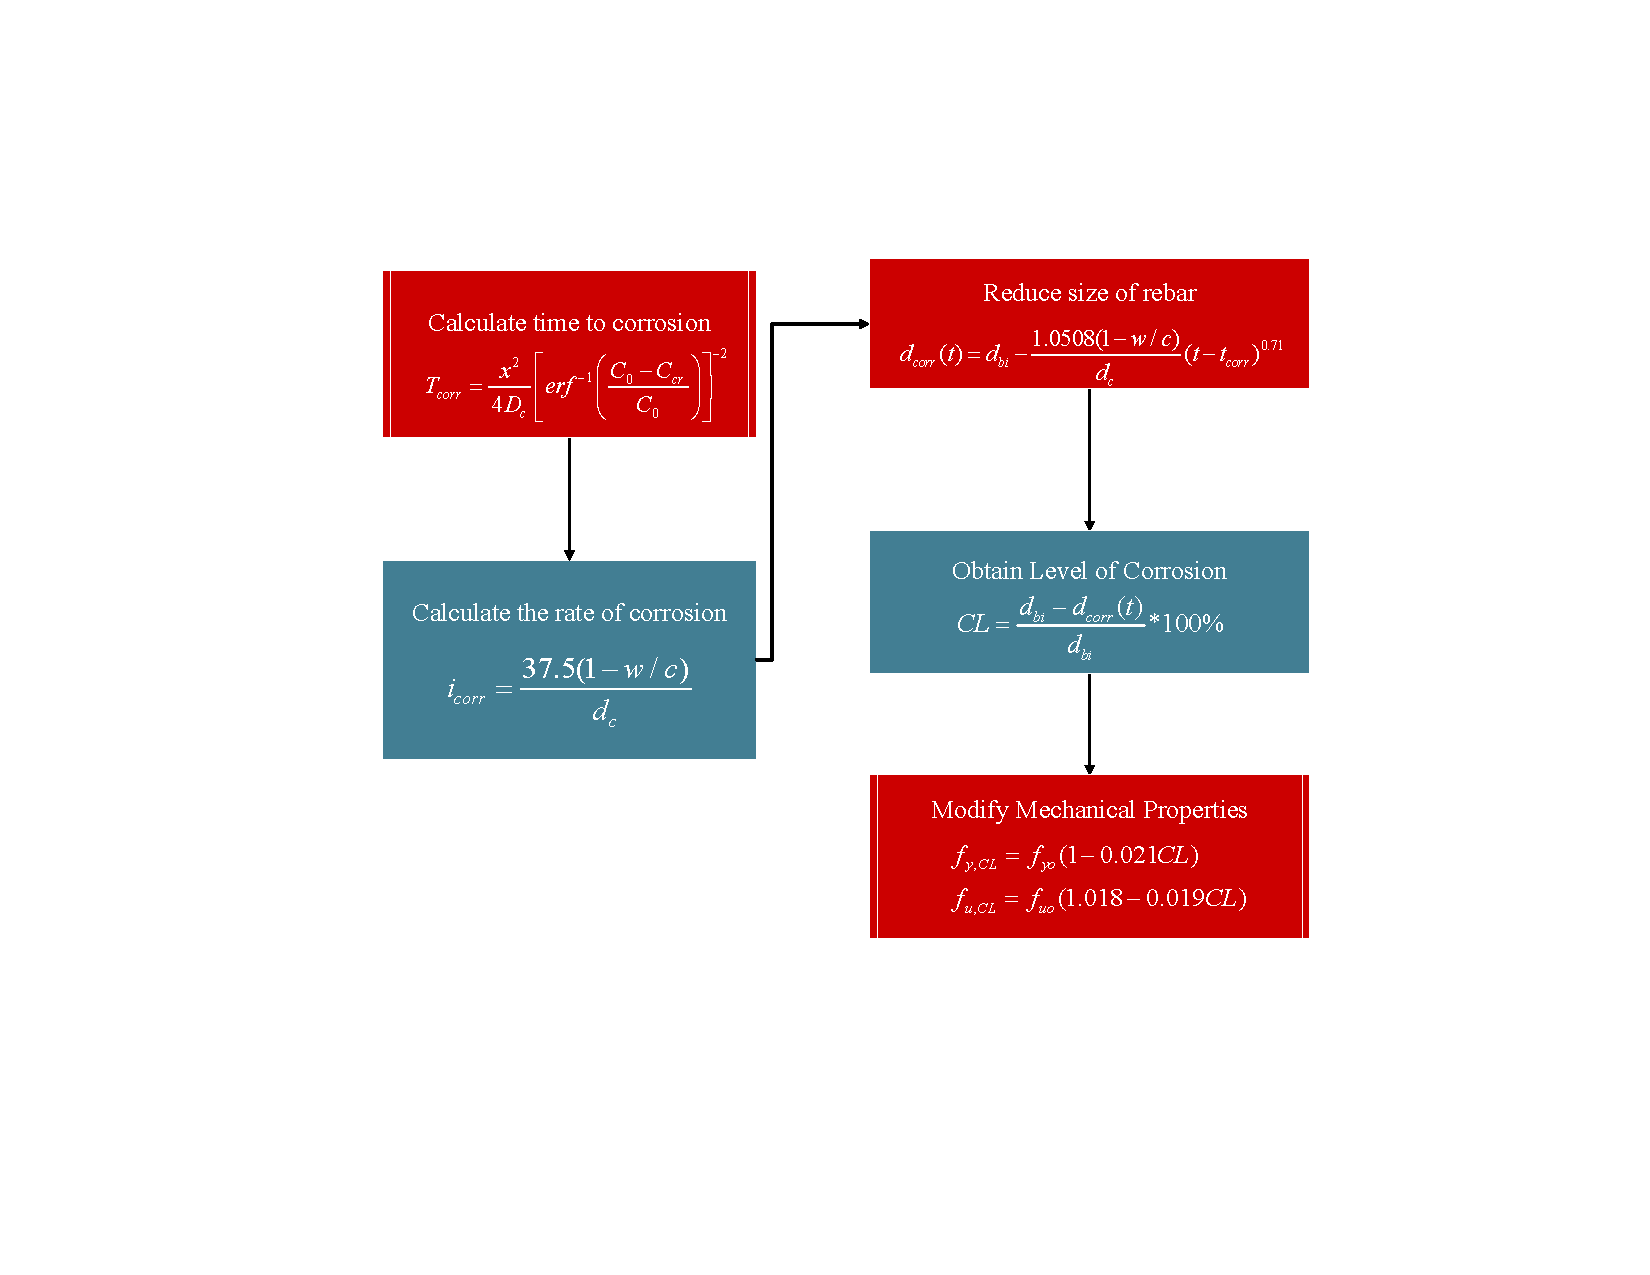
\includegraphics[width=0.7\textwidth]{Chapter-5/figs/Corrosion_Modeling}
	\caption{Corrosion modeling for structural analysis}
	\label{fig:CorrModel}
\end{figure}
%This will be incorporated into the nonlinear structural analysis framework using OpenSeesPy \cite{McKenna2010}\cite{Zhu2018}, the framework of this analysis is explained in section 4.6.
\subsection{Modeling of strain aging for structural analysis}
Strain aging modifies the properties of mild steel after being subjected to large strains, as explained in Chapter \ref{chap-two}. Strain aging is of special relevance in the days following a mainshock. Consider the case of a structure, prone to strain aging, that is subjected to a mainshock and after more than 3 days is subjected to a large aftershock. This structure would behave differently during the aftershock due to the effects of strain aging. This situation is similar to that of the Canterbury Earthquake 2010 - Christchurch Earthquake 2011 sequence, since the ground motions struck in the same area of New Zealand, but occurred 5 months apart. To simulate this case scenario, the model proposed would consist of subjecting a series of SDOF structures to different mainshock-aftershock sequences.  The main variable of study in this case would be the time between the mainshock and the aftershock, and the intensity measure of the ground motions. This procedure is explained in more detail in section 4.2.3. 

\section{Multiple seismic events}

The evaluation of multiple seismic events is a topic that has been scarcely studied, however their effects have been felt in numerous earthquake sequences such as the Christchurch 2010, Umbria-Marche Earthquake 1997 and the Puerto Rico Earthquakes 2020. The hypothesis is that accumulation of damage will restart in a smaller seismic event to achieve a prescribed limit state, similar to how corrosion and other aging phenomena might impact the intensity needed to achieve a future limit state. 

For this study it has been determined that not all damage in structures are dependent on multiple events but rather their condition when an event occurs as is the case for corrosion. Therefore, in this study a Mainshock-Aftershock (MS-AS) sequence is evaluated at different levels of corrosion. Other damage related phenomena, such as strain aging, depend on the loading history and are therefore dependent on the history of extreme loading events. Thus, to study the effect on strain aging a sequences of mainshock-aftershock is focused on the time difference between the mainshock and the aftershock. The outcome will depend on the intensity of the ground motions and the pre-strain value achieved during the mainshock.

\subsection{Earthquake selection}

The earthquake selection will use two approaches to select the ground motions. The first consists of using the PEER web tool to perform amplitude scale matching of records that on average match the design spectrum. The second method involves conditional spectrum matching (CSM), which consists of computing the expected response spectrum associated with a target spectral acceleration ($Sa$) value at a single period, using the information from the probabilistic seismic hazard analysis (PSHA).

In both selection methods it is necessary to define a design spectrum and the PSHA. Therefore, the city of Anchorage, AK is chosen to define the design spectrum and the PSHA.The design spectrum and the data are taken from the USGS PSHA webtool, which is shown in \fref{fig:UHS_AK} and \fref{fig:PSHA_AK}. 

\begin{figure}[htbp]
	\centering
	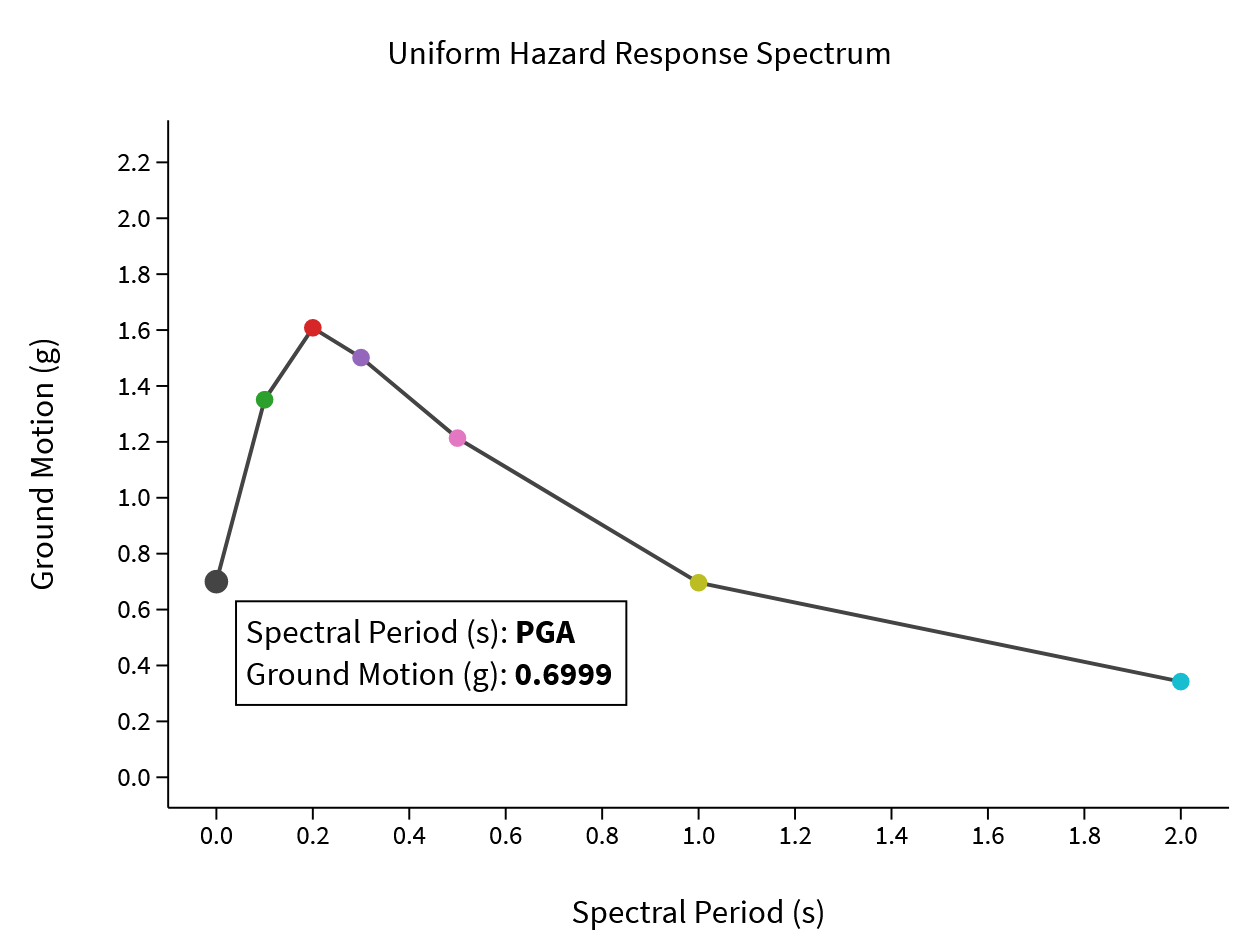
\includegraphics[width=0.75\textwidth]{Chapter-5/figs/UniformHazardResponseSpectrum_AK}
	\caption{Uniform Hazard Spectrum for Anchorage, AK}
	\label{fig:UHS_AK}
\end{figure}

\begin{figure}[htbp]
	\centering
	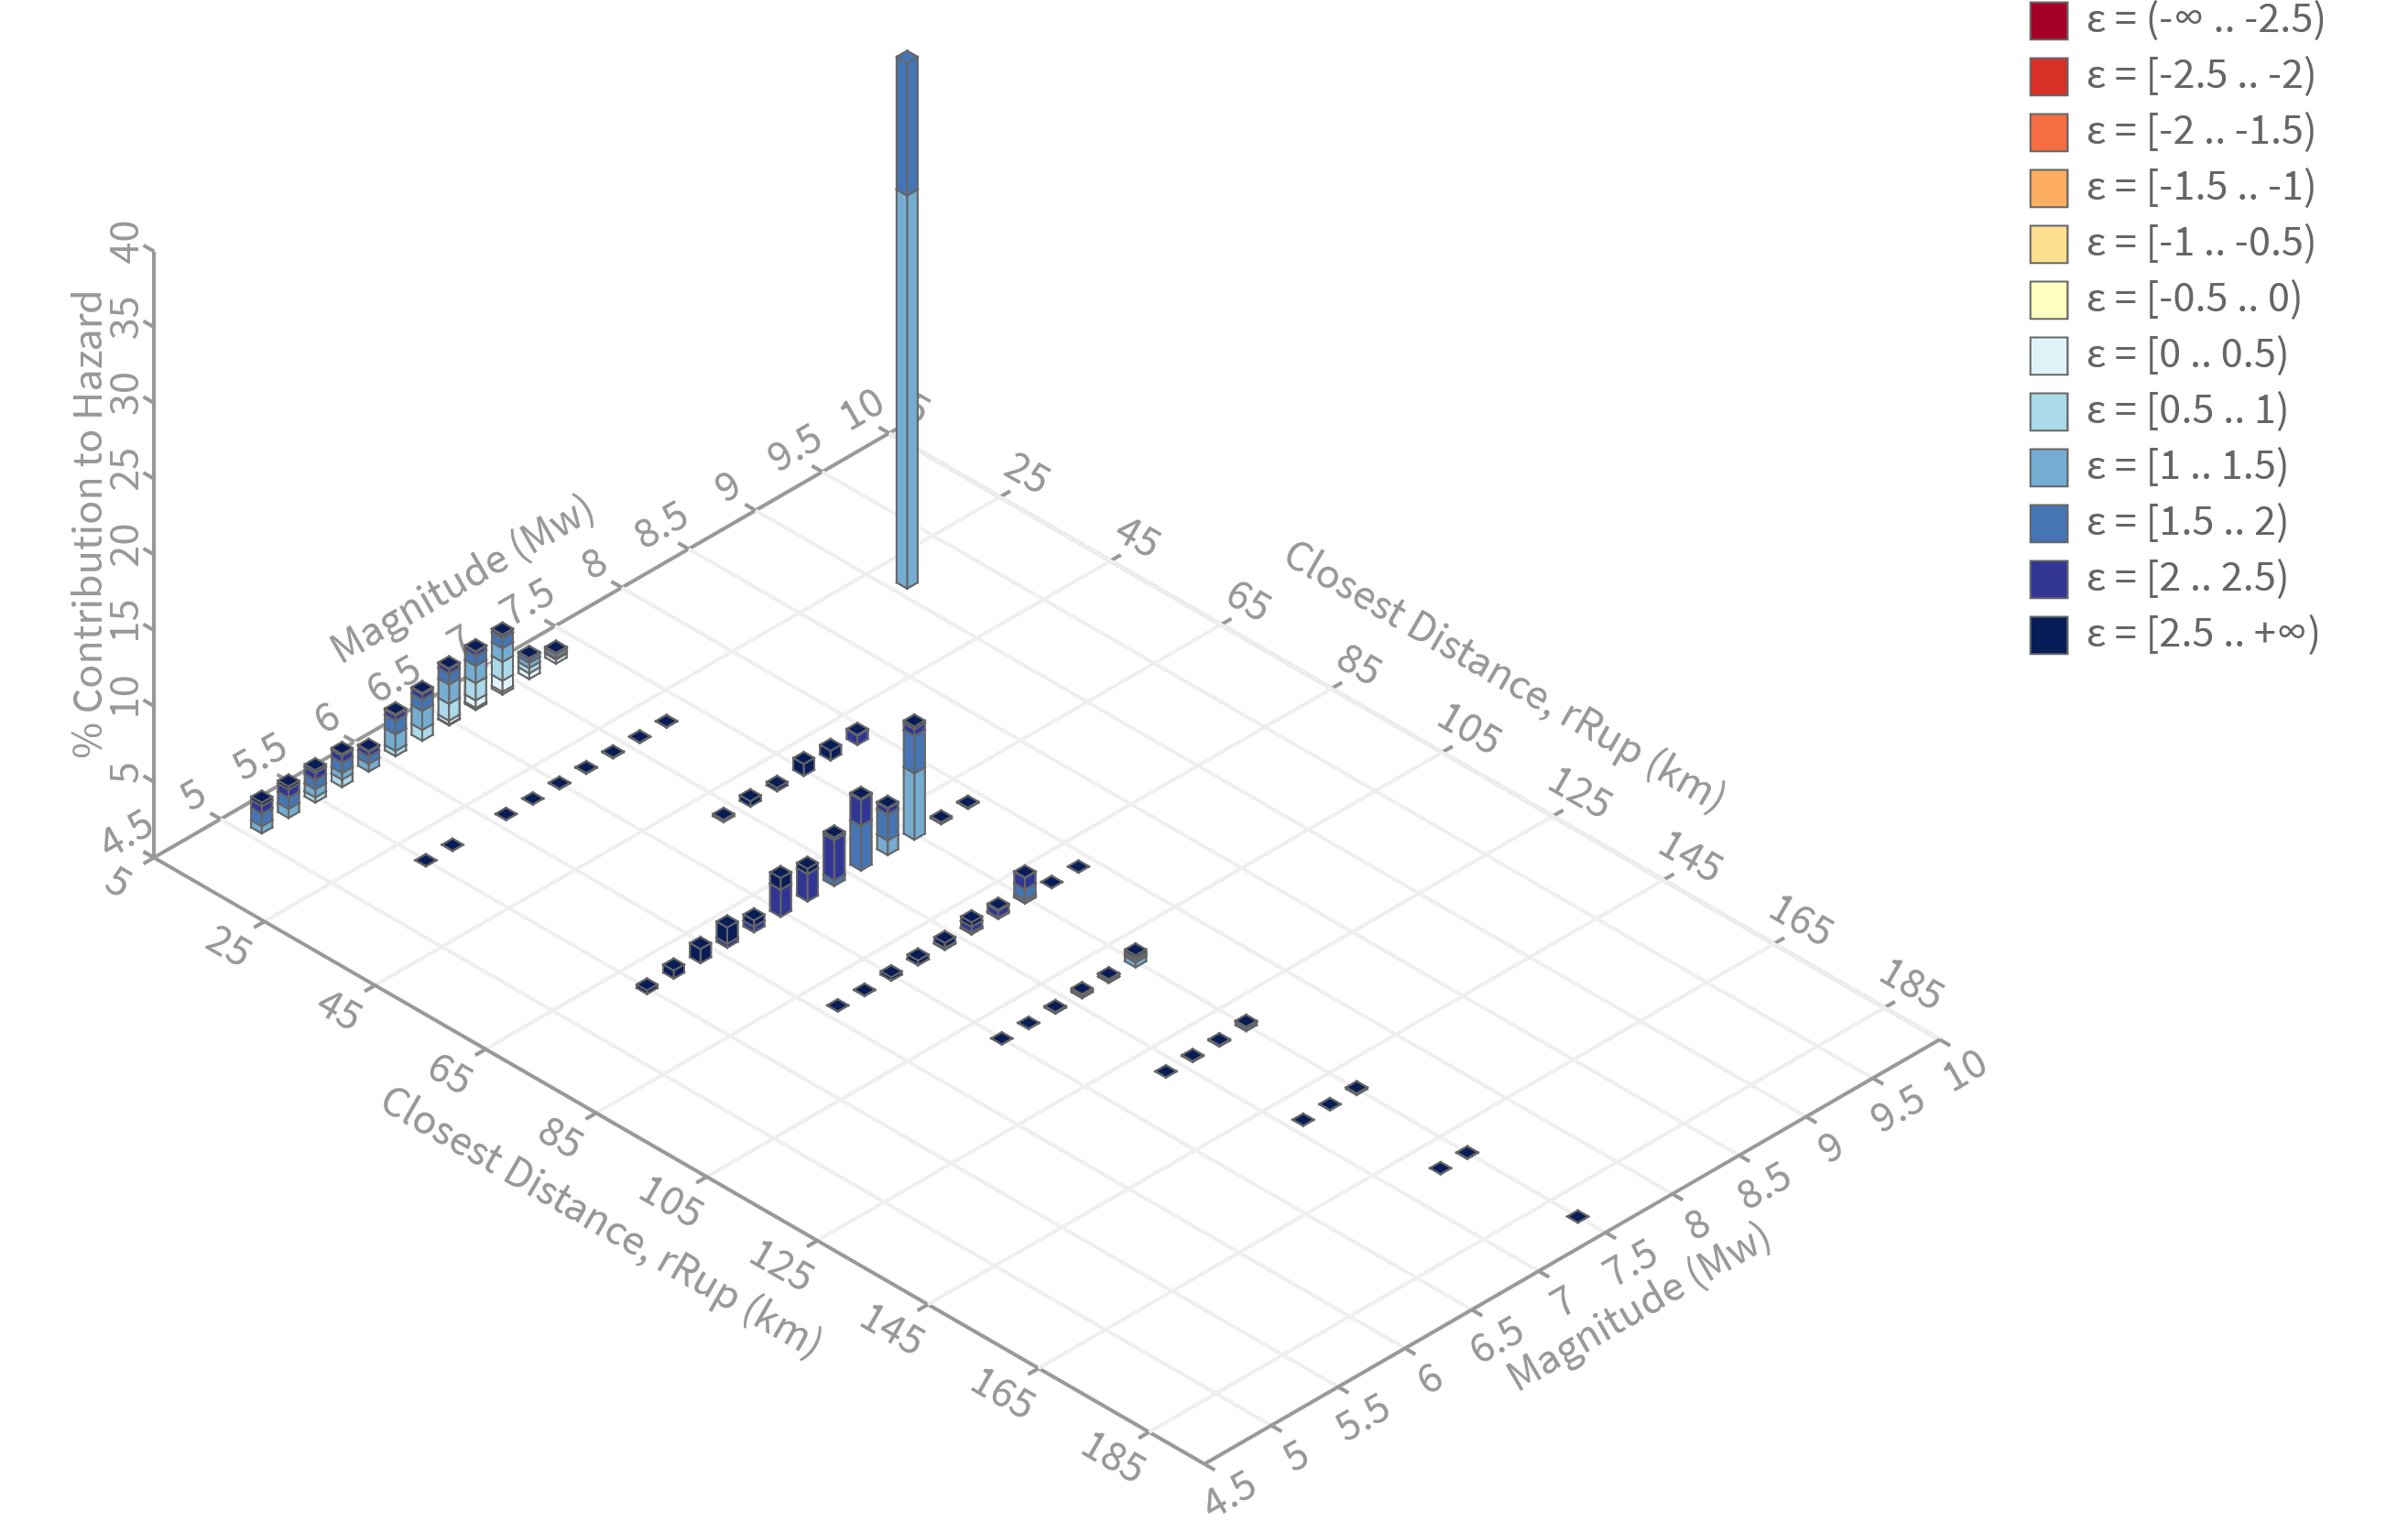
\includegraphics[width=0.6\textwidth]{Chapter-5/figs/PSHA_Deaggregation_Anchorage_AK}
	\caption{PSHA deaggregation for Anchorage, AK}
	\label{fig:PSHA_AK}
\end{figure}
\newpage
The ground motions are taken from the NGA2 West Database of earthquake records provided by the Pacific Earthquake and Engineering Research Institute (PEER) \cite{Ancheta2014}. This database consists of 599 different earthquake events that characterize the ground motions on the west coast of the contiguous United States. The data was filtered according to the following criteria:

\begin{itemize}
	\item Must be a mainshock-aftershock sequence
	\item Moment magnitude $M_w \geqslant 5$
	\item $PGA>0.04$
	\item $PGV>1$ cm/s
	\item $Vs_{30}>100m/s$ \& $Vs_{30}<1000$ m/s
	\item Lowest usable frequency is less than 1Hz
	\item $R_{rup}<60km$
\end{itemize}

Figure \ref{fig:MS_Selection} summarizes the results from filtering the data available in the PEER NGA West2 database. \fref{fig:MS_Selection} shows the earthquakes as moment magnitude {Mw} vs rupture distance ($R_{rup}$).

%\begin{itemize}
%	\item Managua
%	\item Northridge
%	\item Duzce 
%	\item Mammoth lake
%\end{itemize}

\begin{figure}[htbp]
	\centering
	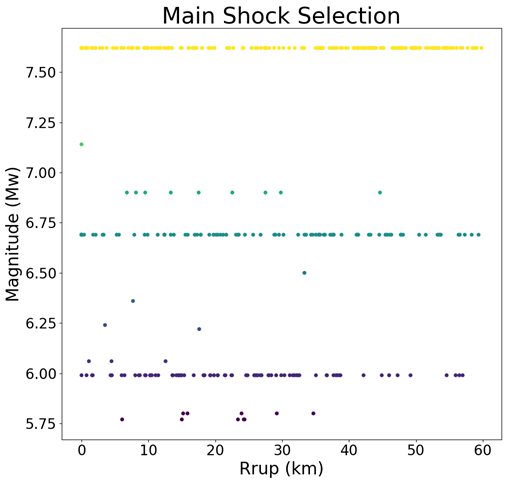
\includegraphics[width=0.6\textwidth]{Chapter-5/figs/MainShock_Selection}
	\caption{Mainshock selection from PEER NGA West2 database}
	\label{fig:MS_Selection}
\end{figure}

\subsection{Modeling of mainshock-aftershock series for corrosion damage state}
Corrosion modifies the mechanical properties of rebars in RC structures, thus inherently modifying their response to earthquake loading. When an earthquake will occur is difficult to predict as explained in section 2.4.2. Therefore, in this study we propose subjecting structures at a specified corrosion level to a series of mainshock and aftershock ground motions. The proposed methodology will help to evaluate the effect of corrosion in RC structures subjected to earthquake loading with accumulation of damage. 
Specifically, the approach consists of (1) specify corrosion level (CL) as shown in \fref{fig:CorrModel}, (2) the ground motions sequences from earthquake selection are applied for each corrosion level, (3) the results are evaluated in each case to determine what limit states were reached and the implication for the design proposal. 


\subsection{Modeling of mainshock-aftershock series for strain aging damage state}

Strain aging consists of the increase in strength of steel after time has passed between a large strain and the new loading. It is possible that structures after being subjected to a mainshock develop the strain aging condition, especially if the maximum strain was higher than $2\varepsilon_{y}$. Therefore, the main variable of study for strain aging condition is the time between the main loading and the secondary loading. It is thus evident that the variable of study for strain aging is the time gap between the mainshock and the aftershock. 

The proposed modeling of the mainshock-aftershock sequence in for strain aging consists of (1) the structure is subjected to the main shock, and the maximum strain in the rebar is recorded, (2) the time gap between the mainshock and the aftershock is varied between 3 days thorugh 50 days, (3) the mechanical properties of the rebar are modified according to \eref{eq.twelve} through \eref{eq.fourteen}, (4) the structure is evaluate for the aftershock groundmotion, and (5) the results are evaluated in each case to determine what limit states were reached and the implication for the design proposal.

\begin{figure}[htbp]
	\centering
	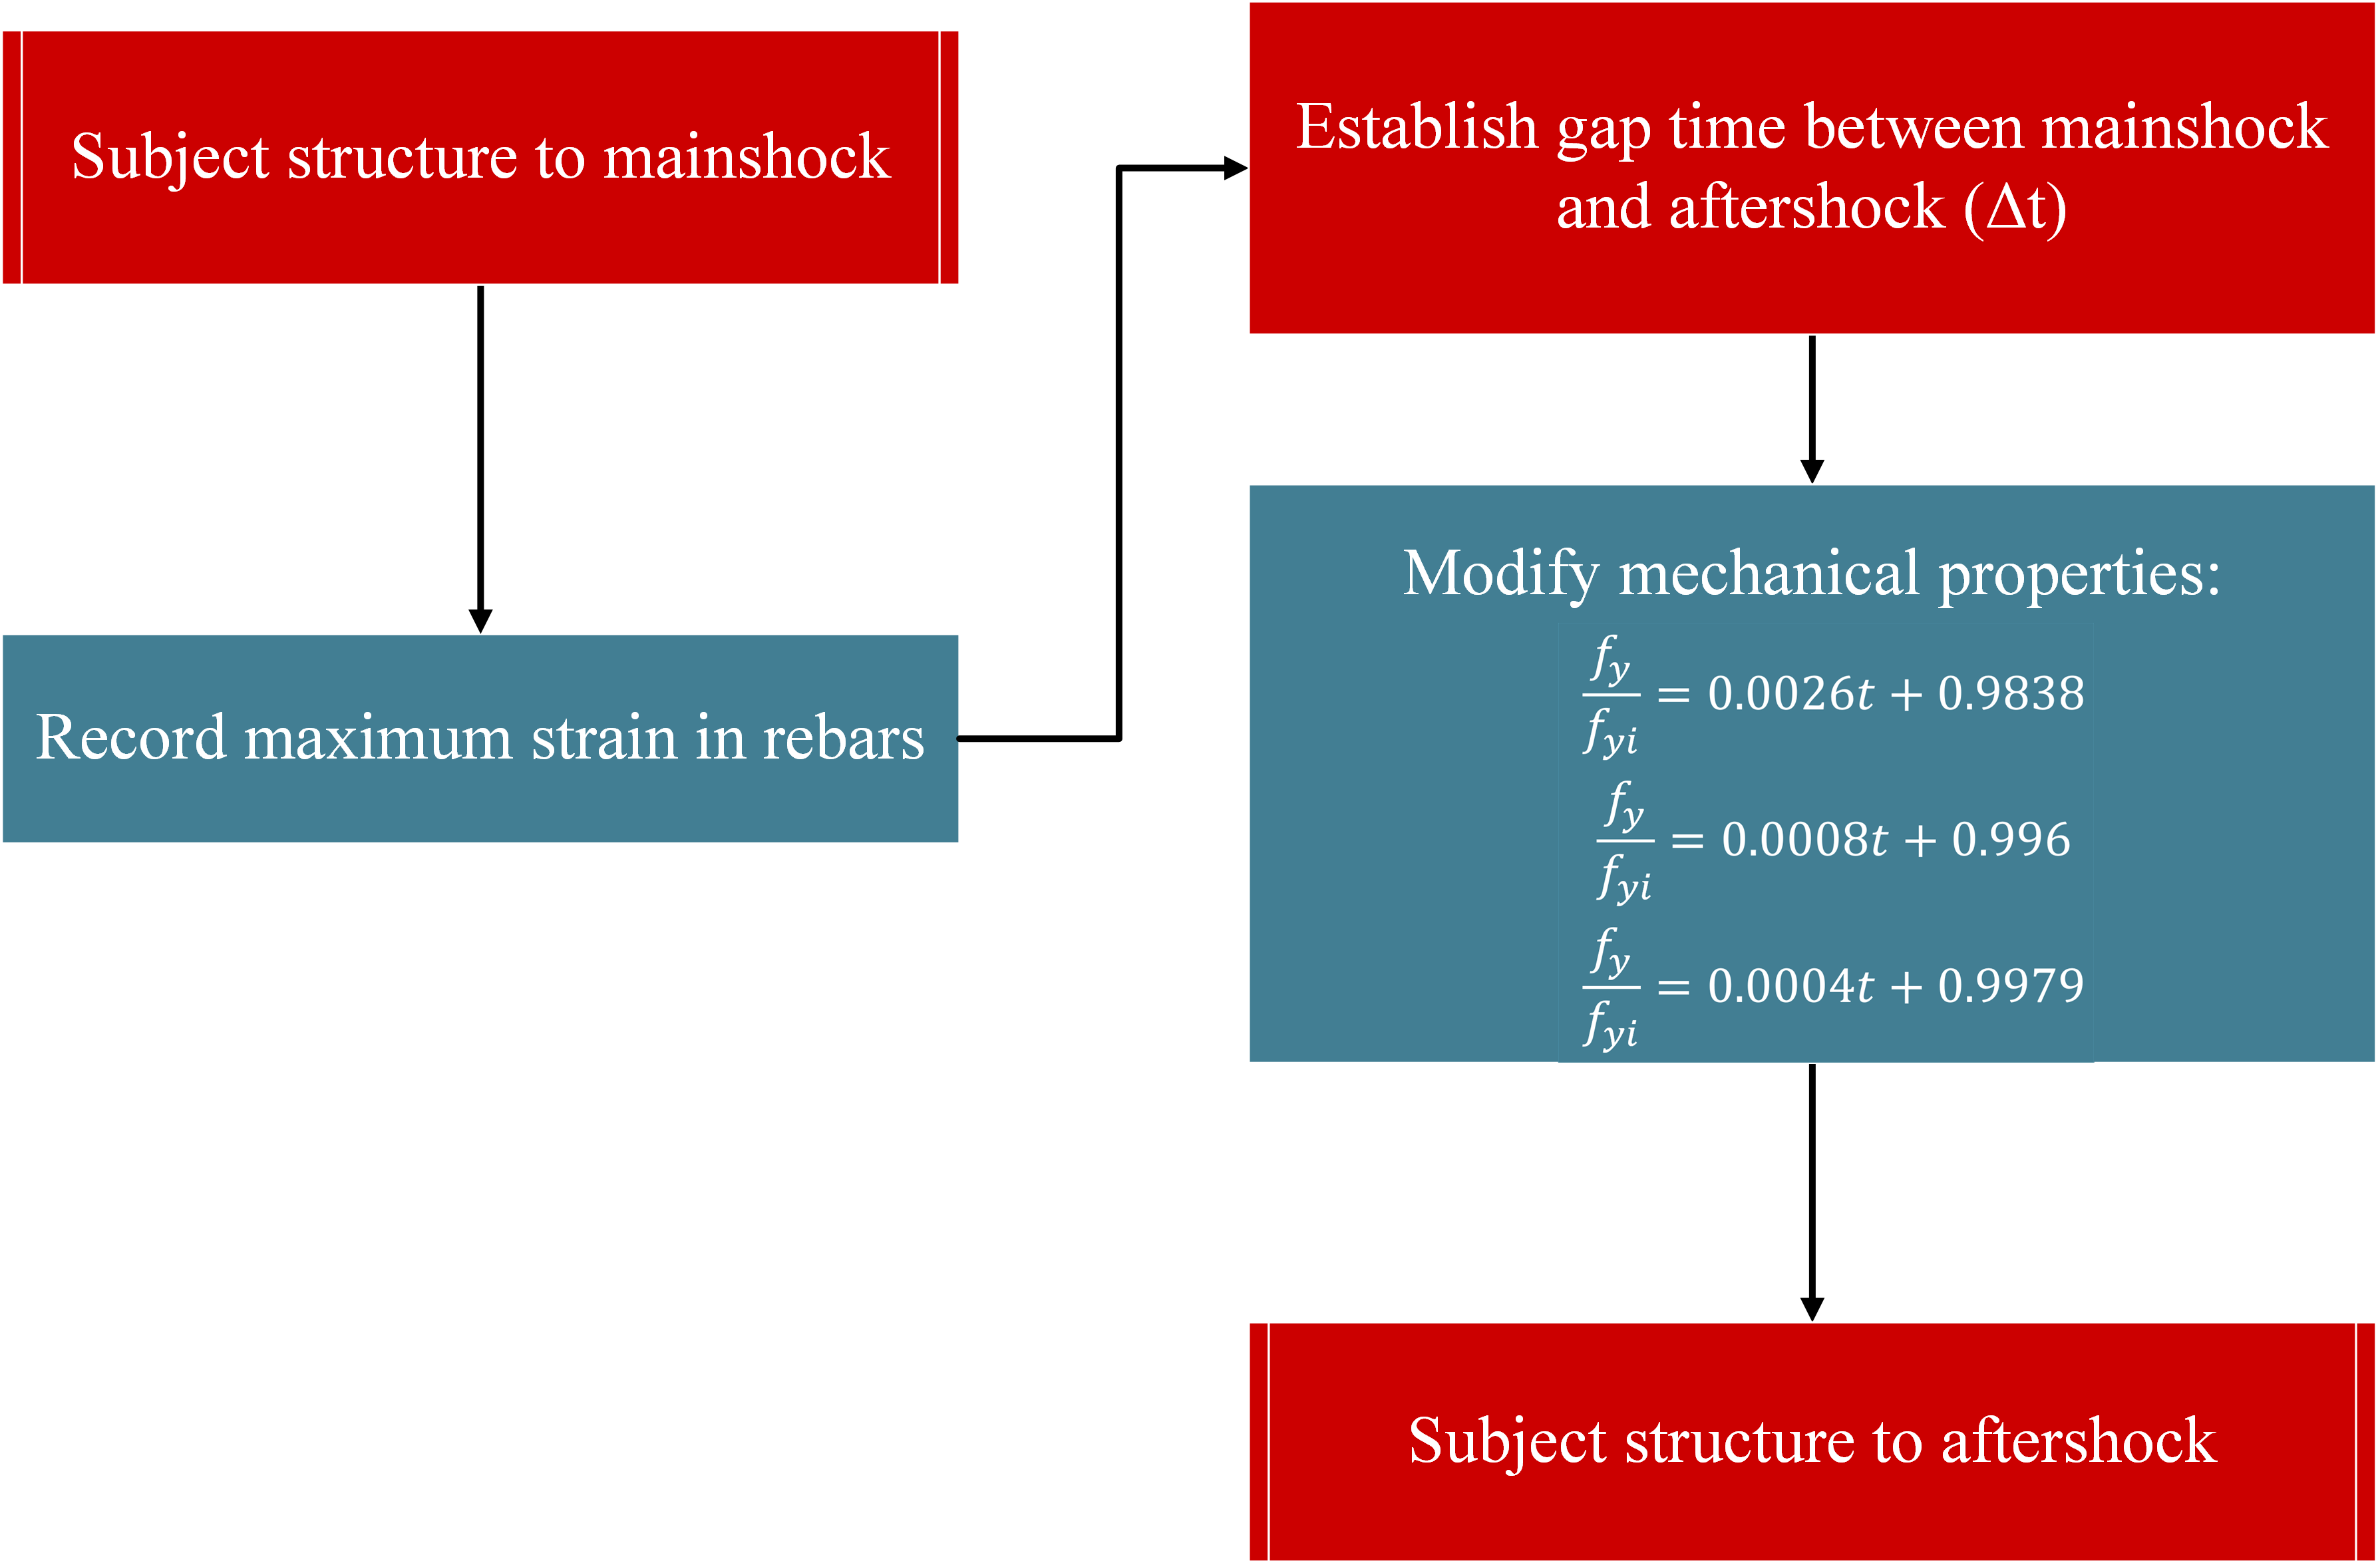
\includegraphics[width=0.9\textwidth]{Chapter-5/figs/StrainAgeing_Modeling}
	\caption{Mainshock-aftershock modeling for strain aging}
	\label{fig:AgingModel}
\end{figure}

\newpage
\section{Analytical Model}

\subsection{Cantilever column}
This study focuses on the behavior of a single degree of freedom (SDOF) system representing a cantilever reinforced concrete column. The column is modeled as shown in \fref{fig:Structural_Model} This structure is modeled in OpenSeesPy \cite{McKenna2010}\cite{Zhu2018} using the $forceBeamColumn$ element \cite{Scott}. The forceBeamColumn element is used with two-point Gauss-Radau integration applied in the hinge regions and two-point Gauss integration applied on the element interior for a total of six integration points \cite{Scott}. The force-based formulation requires only a single element to accurately represent the full nonlinear deformation of the member and the integration scheme selected prevents the loss of objectivity during the softening response while also providing integration points at the member ends \cite{Calabrese2010},\cite{Scott}. The element requires the length of plasticity be defined at each end of the member, for which the tension-based rectangular plastic hinge length is calculated using the following expressions \cite{Goodnight2013}:

\begin{equation}
    L_{pc}=k*L_{eff} + 0.4D
    \label{eq:LP_Comp}
\end{equation}
\begin{equation}
	k=0.2*(Fu/Fy - 1) \leqslant 0.08
	\label{eq:K_Lp}
\end{equation}
\begin{equation}
    L_{pt}=L_{pc}+\gamma*D
    \label{eq:LP_Tension}
\end{equation}

For single bending the parameter $\gamma$ is:
\begin{equation}
    \gamma=0.33
    \label{eq:Gamma_LPt}
\end{equation}

The two-point Gauss-Radau integration is applied such that each end node integration is weighted equal to the specified plastic hinge length, as illustrated in \fref{fig:Fiber_PlasticHinge}. In this figure $D$ is the diameter of the column, and $c$ is the concrete cover. Therefore, strains recorded at the end sections represent accurate values even in the case where deformation localizes to the ends from strain-softening behavior. For the case of the cantilever column considered, only one plastic hinge length is defined, and the opposite end is given an arbitrary unit length. 

\begin{figure}[htbp]
	\centering
	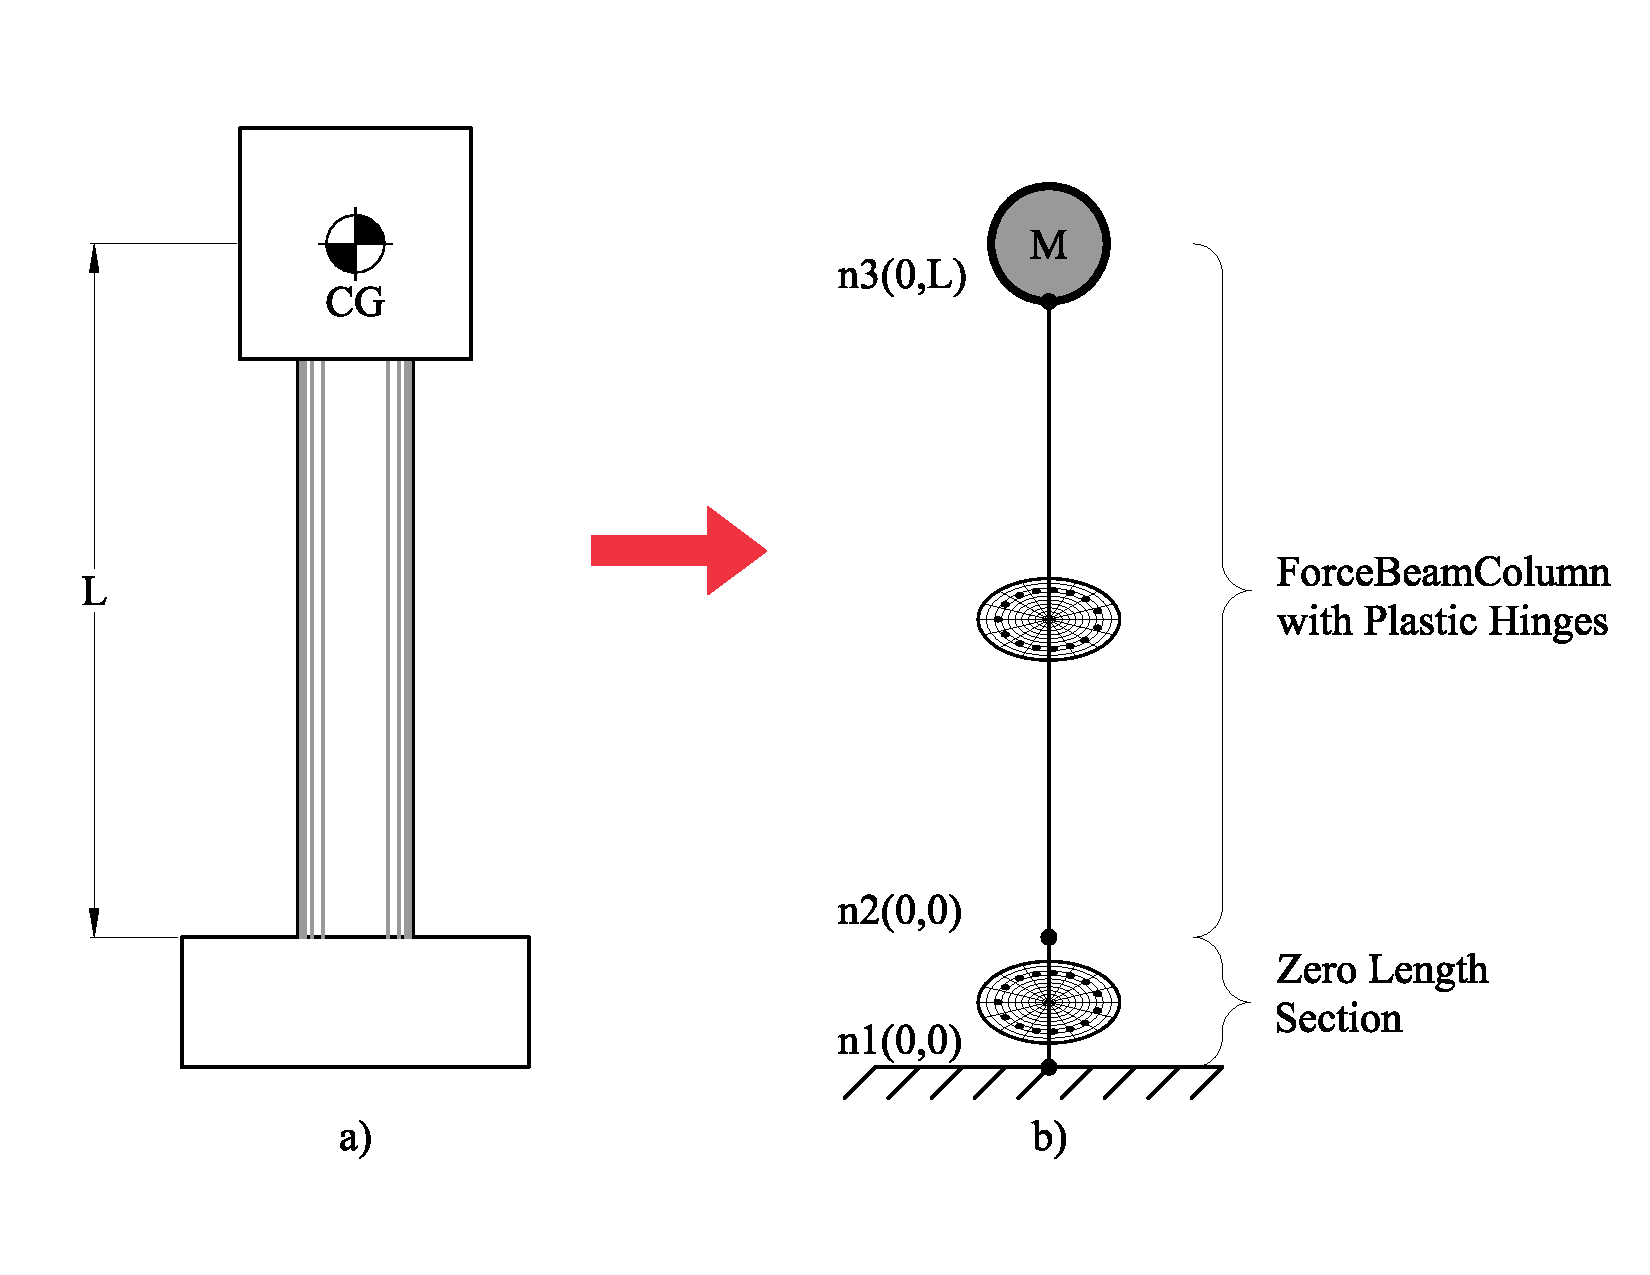
\includegraphics[width=0.75\textwidth]{Chapter-5/figs/StructuralModel_01}
	\caption{Structural Model a) SDOF Column b) Structural Model}
	\label{fig:Structural_Model}
\end{figure}

\begin{figure}[htbp]
	\centering
	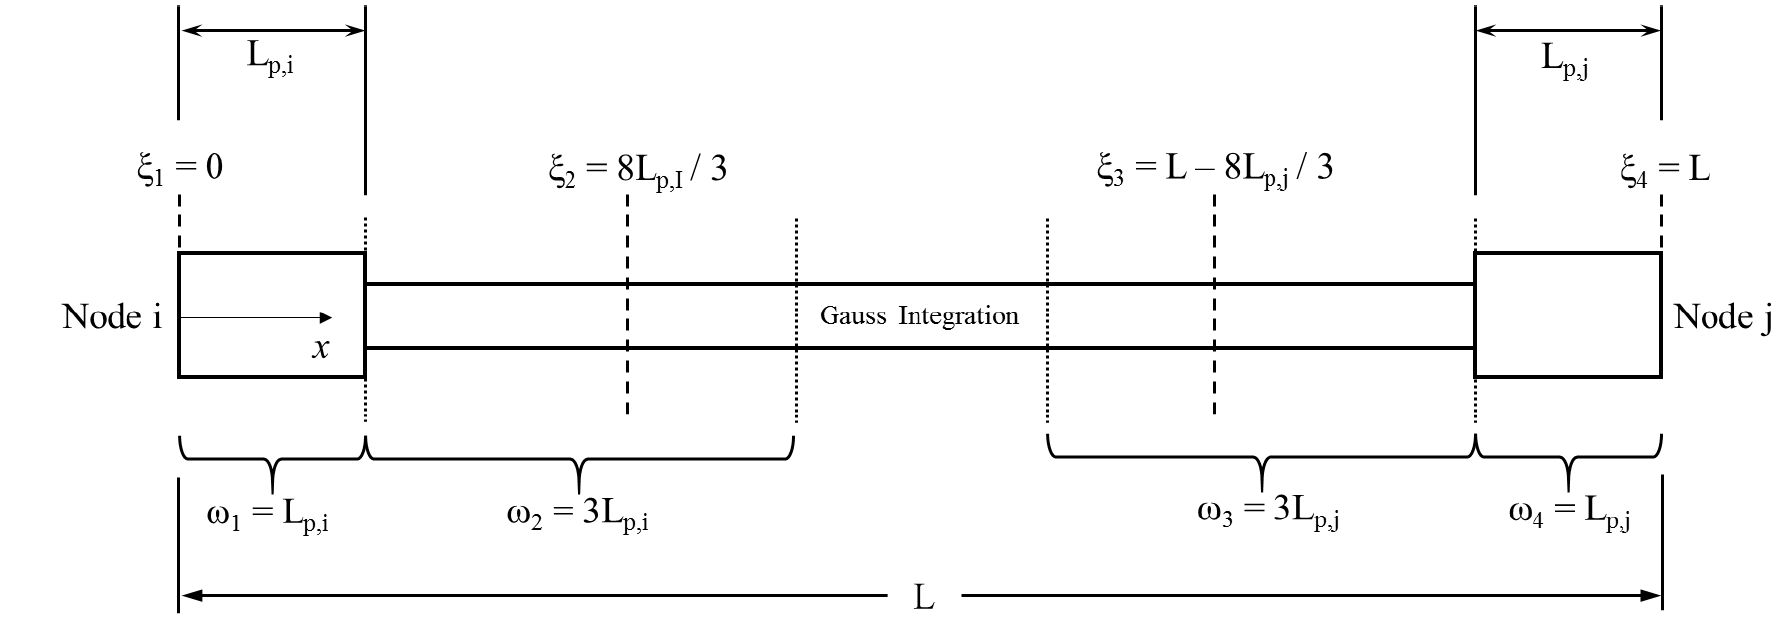
\includegraphics[width=0.9\textwidth]{Chapter-5/figs/fbc_PlasticHinge}
	\caption{End point plastic hinge method \cite{Scott}}
	\label{fig:Fiber_PlasticHinge}
\end{figure}

The cross section of the column is shown in \fref{fig:ColumnSection}. The column cross section is discretized with concrete and steel material fibers. Concrete fibers are modeled using the $Concrete01$ material, modified for confined material strength based on the Mander confined concrete model \cite{Mander1988}. The $Steel02$ material, based on the Giuffre-Menegotto-Pinto model \cite{Filippou1983} is used for the longitudinal reinforcement with recommended parameters ($b = 0.01, R0 = 20, cR1 = 0.925, cR2 = 0.15$). 

\begin{figure}[htbp]
	\centering
	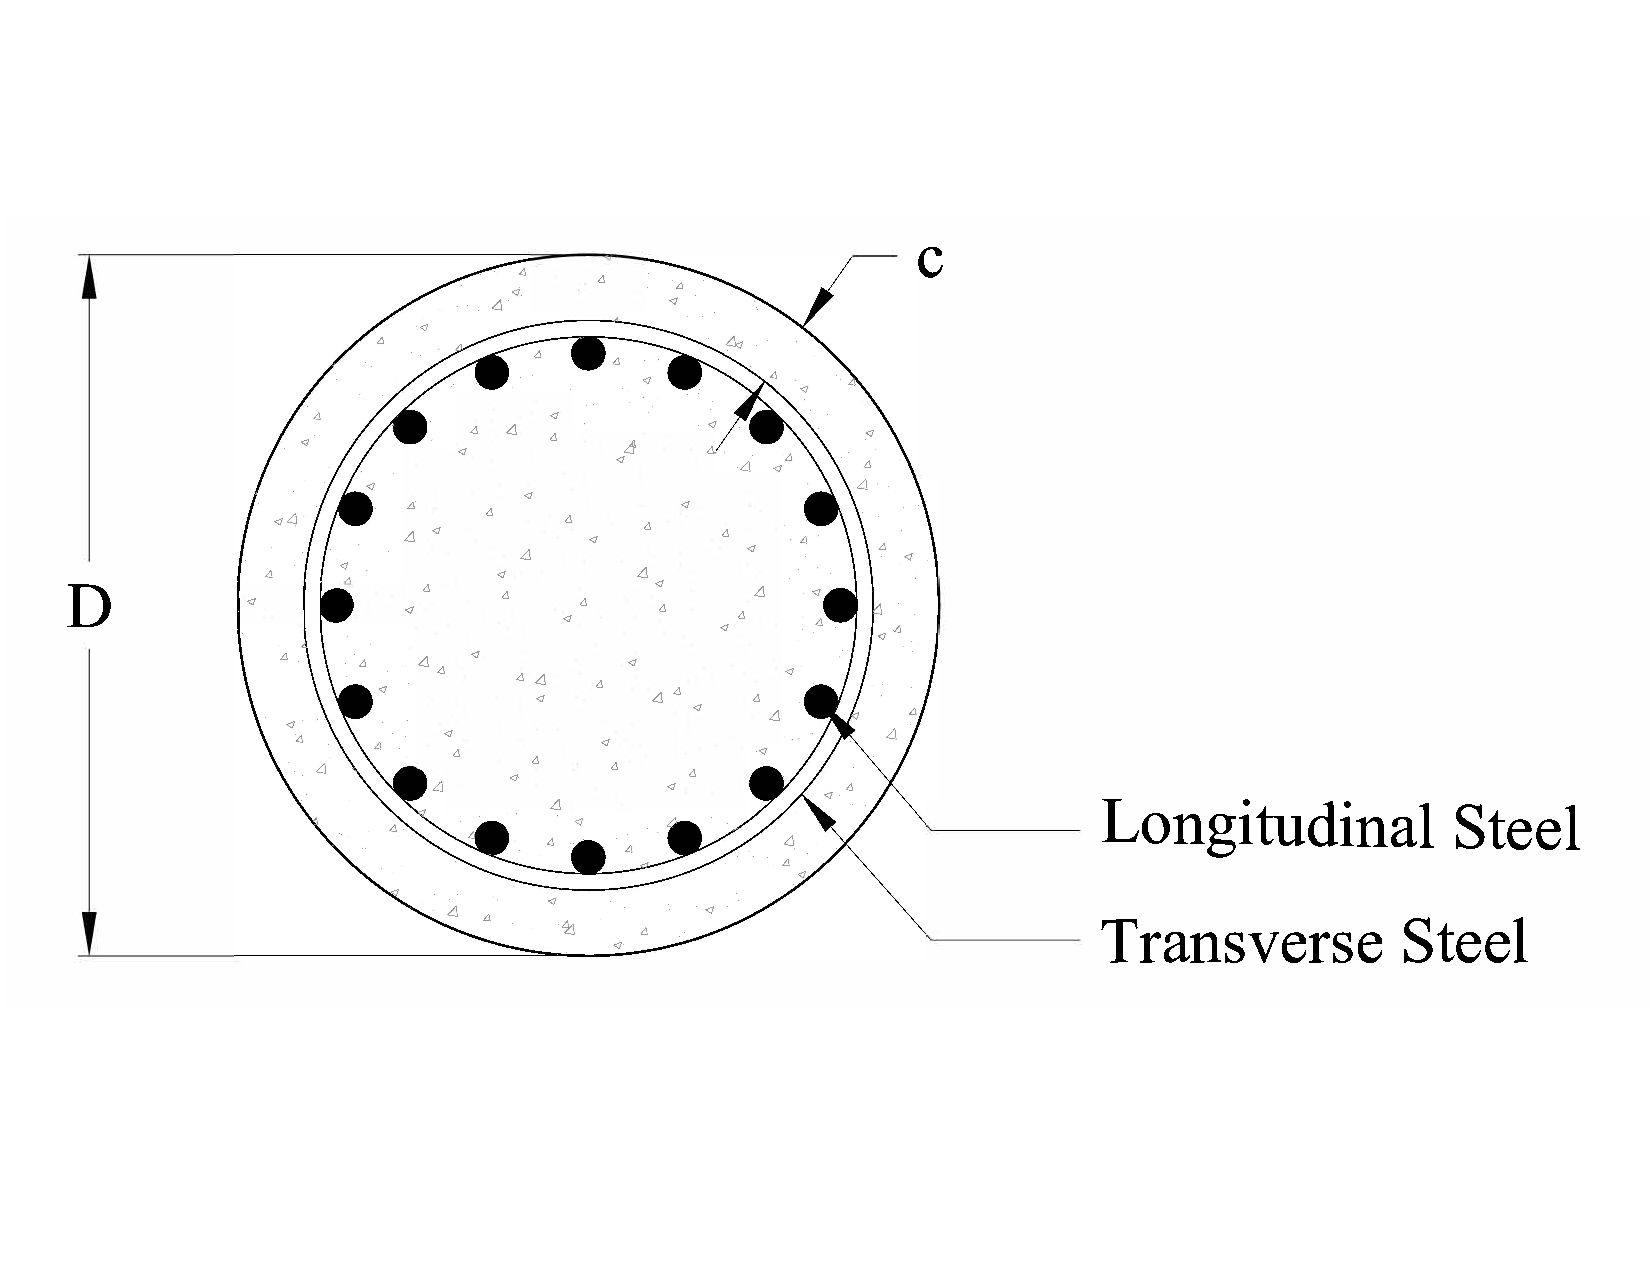
\includegraphics[width=0.7\textwidth]{Chapter-5/figs/StructuralModel_Section}
	\caption{Section of the RC Column}
	\label{fig:ColumnSection}
\end{figure}
\subsection{Strain penetration}

The strain penetration considers the additional deformation due to anchorage of the reinforcement into the foundation, since tension strain in the reinforcement will drop to zero at a depth equal to the true development length of the rebar \cite{Priestley2007}. Experimental studies have generally reported that this end rotation contributes up to 35\% to the lateral deformation of flexural members\cite{Zhao2007}. Therefore, it is important to incorporate it into the analytical model. A way to capture this effect is by using a zero-length section element implemented in the nonlinear fiber-based analysis of concrete structures, which is available in the material library of OpenSeesPy as $Bond SP1$ \cite{Zhao2007}. This is the material model used for the steel fibers of the zero-length section element.

The required parameters for this model are:
\begin{itemize}
	\item $F_{y}$ Yield strength of the reinforcement steel
	\item $S_{y}$ Rebar slip at member interface under yield stress (see \eref{eq.Rebar_Slip})
	\item $F_{u}$ Ultimate strength of the reinforcement steel
	\item $S_{u}$ Rebar slip at the loaded end at the bar fracture strength a value of $35 S_{y}$ is recommended \cite{Zhao2007}
	\item $b$ Initial hardening ratio in the monotonic slip vs. bar stress response $b=0.45$ is recommended \cite{Zhao2007}
	\item $R$ Pinching factor for the cyclic slip vs. bar response $R=1.01$ is recommended \cite{Zhao2007}
	\item $d_b$ Rebar diameter
	\item $f'c$ Concrete compressive strength of the adjoining connection member
	\item $\alpha$ Parameter used in the local bond-slip relation and can be taken as $\alpha=0.4$ in accordance with CEB-FIP Model Code 90 \cite{CEB1993}
\end{itemize}.
\newline
Bar slip is calculated as:
\begin{equation}
	S_{y}(in)=0.1\left(\frac{d_{b}F_{y}}{4000\sqrt{f'_{c}}}\left(2\alpha+1\right)\right)^{\frac{1}{\alpha}}+0.013 (in)
	\label{eq.Rebar_Slip}
\end{equation}
\subsection{Design limit states}
Design limit states are defined based on strains in the material since they can more accurately represent the different performance levels of a structure. Structure limit states are defined as tension strains in the rebars or compression strains in the concrete core. The values recommended in typical performance-based design of reinforced concrete bridge columns are shown in Table  \ref{tab:DesignLimitStates}. The serviceability limit states correspond to the compression strain at which concrete cover begins to crush and the peak tension strain which results in residual crack widths of approximately 1 mm. These limits are generally accepted as nominal limit states for RC members. The compression limit state for damage control is defined by the expression shown in Eq. \ref{eq:ec_DamageControl}, and it refers to the compression strain in the confined concrete at which fracture of the transverse reinforcement confining the core occurs \cite{Priestley2007}. This equation is obtained using the strain-energy balance between that absorbed by the confined core concrete and the capacity of the confining steel. The tension damage control limit state is defined by the strain at the onset of buckling which can be expressed according to \ref{eq:es_DamageControl}. This model demonstrated accurate predictions of the onset of bar buckling on physical tests in SDOF Concrete Column \cite{Goodnight2016}. The bar buckling limit state could change as a result of the experimental campaign proposed in Chapter 4.

\begin{equation}
    \varepsilon_{c,spiral yield}=0.009-0.3\frac{A_{st}}{A_{g}} +3.9\frac{f_{yhe}}{E_{s}}
    \label{eq:ec_DamageControl}
\end{equation}

\begin{equation}
    \varepsilon_{s,BB}=0.03+700\rho_{s}  \frac{f_{yhe}}{E_{s}} -0.1\frac{P}{f'_{c}A_{g}}
    \label{eq:es_DamageControl}
\end{equation}


\begin{table}[htbp]
	\caption{Design limit states}
	\label{tab:DesignLimitStates}
	\centering	
		\begin{tabular}{|l|c|c|}
		\hline
		\cellcolor[HTML]{CC0000}{\color[HTML]{FFFFFF}Limit State} & \cellcolor[HTML]{CC0000}{\color[HTML]{FFFFFF}Concrete Limit State $\varepsilon_{c} (in/in)$} & \cellcolor[HTML]{CC0000}{\color[HTML]{FFFFFF}Reinforcing Steel Limit State $\varepsilon_{s} (in/in)$}\\  \hline	
		Serviceability       & 0.004                           & 0.015  \\  \hline	
		Damage Control       & Eq. \ref{eq:ec_DamageControl}   & Eq. \ref{eq:es_DamageControl}\\  \hline
		\end{tabular}
\end{table}
 
\section{Comparison with existing physical tests}
The model used in this research is calibrated for the case of pristine conditions and the case of corroded columns. The calibration to a pristine condition column shows how reliable the results from the model are. Then the pristine condition model is modified with the corrosion model, as explained in section 4.1.1. The analytical model is compared to the results from the physical test on corroded RC columns. This will give confidence that the results obtained from the analytical model are reliable, and will be further enhanced with the experimental results.
\subsection{Pristine condition columns}
Goodnight et al performed a total of 30 circular RC columns quasi-static tests to evaluate strain limit states \cite{Goodnight2016}. From this set of tests, a sample of one was taken to calibrate the analytical model. The test performed by Goodnight et al on an SDOF cantilever column shows similar geometry to that presented in \fref{fig:Fiber_PlasticHinge}. The parameters used in this large scale test were: diameter $D = 24.0 inch$, height of the column $L = 8.0 ft$, yield strength of steel $f_{y} = 574.0 MPa$, ultimate strength of steel $f_{u} = 753.3 * MPa$, longitudinal steel volumetric ratio $\rho_{s} = 1.5\% $, transverse steel volumetric ratio $\rho_{v} = 1.0\% $, and strength of concrete at 8 days $f'_{c} = 39.8 MPa$.

The analytical model used these parameters to compare the results from the model to the experimental results. The results from the analysis show good agreement with the experimental results as evidenced in \fref{fig:ModelCalibration}. Thus, the results obtained from the model predict the overall system behavior and can be used to analyze other configurations of the structural model.
\begin{figure}[htbp]
	\centering
	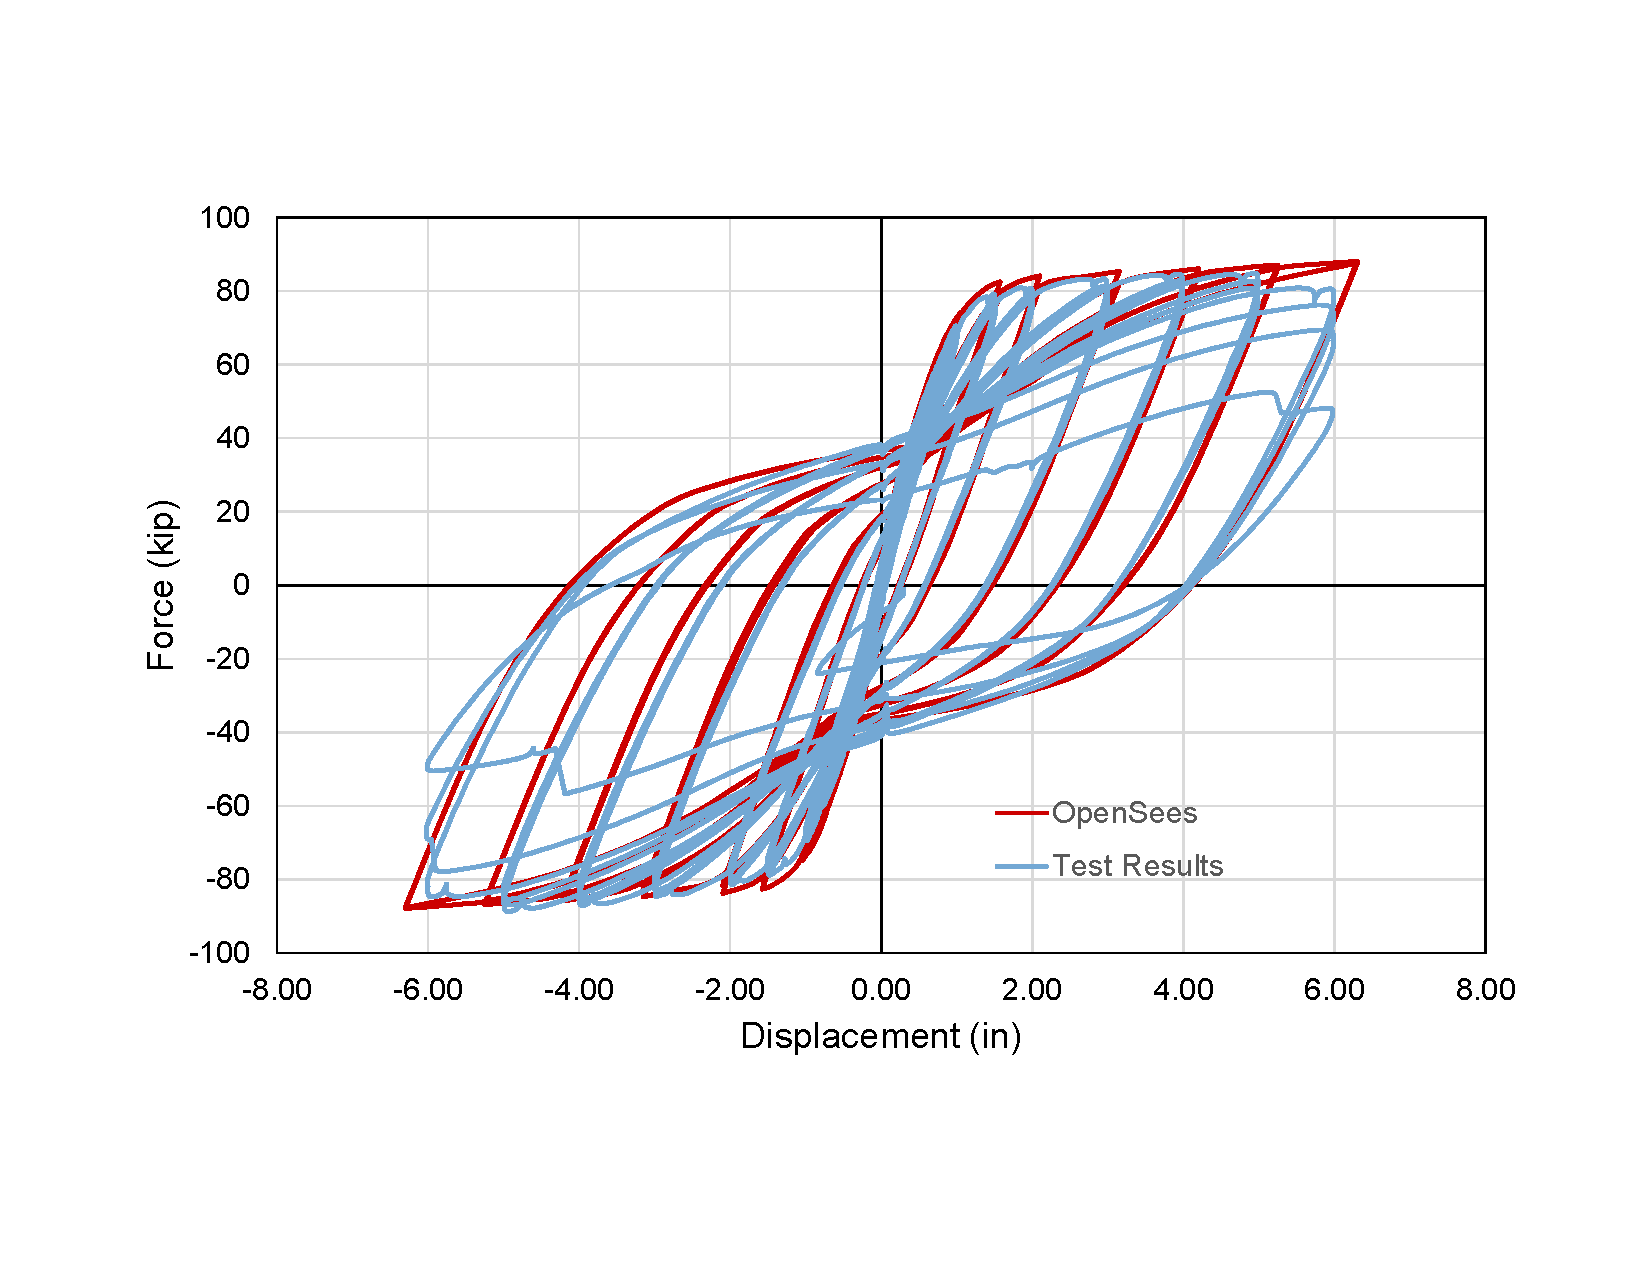
\includegraphics[width=0.6\textwidth]{Chapter-5/figs/Model_Calibration_Goodnight2016}
	\caption{Force-Displacement results from experimental results \cite{Goodnight2013} and analytical model}
	\label{fig:ModelCalibration}
\end{figure}
\newpage

\subsection{Accelerated corrosion columns}
Similarly, Ma et al performed a series of quasi-static tests on RC columns with different corrosion levels and axial load ratios \cite{Ma2012}. From their study, the test with a corrosion level $CL=9.5\%$ was taken for calibration since the other tests presented in their study had excessively high axial load ratios which are not common in RC bridges. The results from Ma et al test	\cite{Ma2012} were used to compare against the analytical model. The column had the following parameters: diameter $D = 260.0 mm$, height of the column $L = 820.0 mm$, yield strength of steel $f_{y} = 375.0$ MPa, ultimate strength of steel $f_{u} = 572.3$ MPa, longitudinal steel volumetric ratio $\rho_{s} = 1.5\% $, transverse steel volumetric ratio $\rho_{v} = 1.0\% $, strength of concrete at 8 days $f'_{c} = 39.8$ MPa, and corrosion level $CL=9.5\%$. Equation \ref{eq.eleven} is used to modify the material properties of the reinforcing steel and considers the effects of corrosion. 

\begin{figure}[htbp]
	\centering
	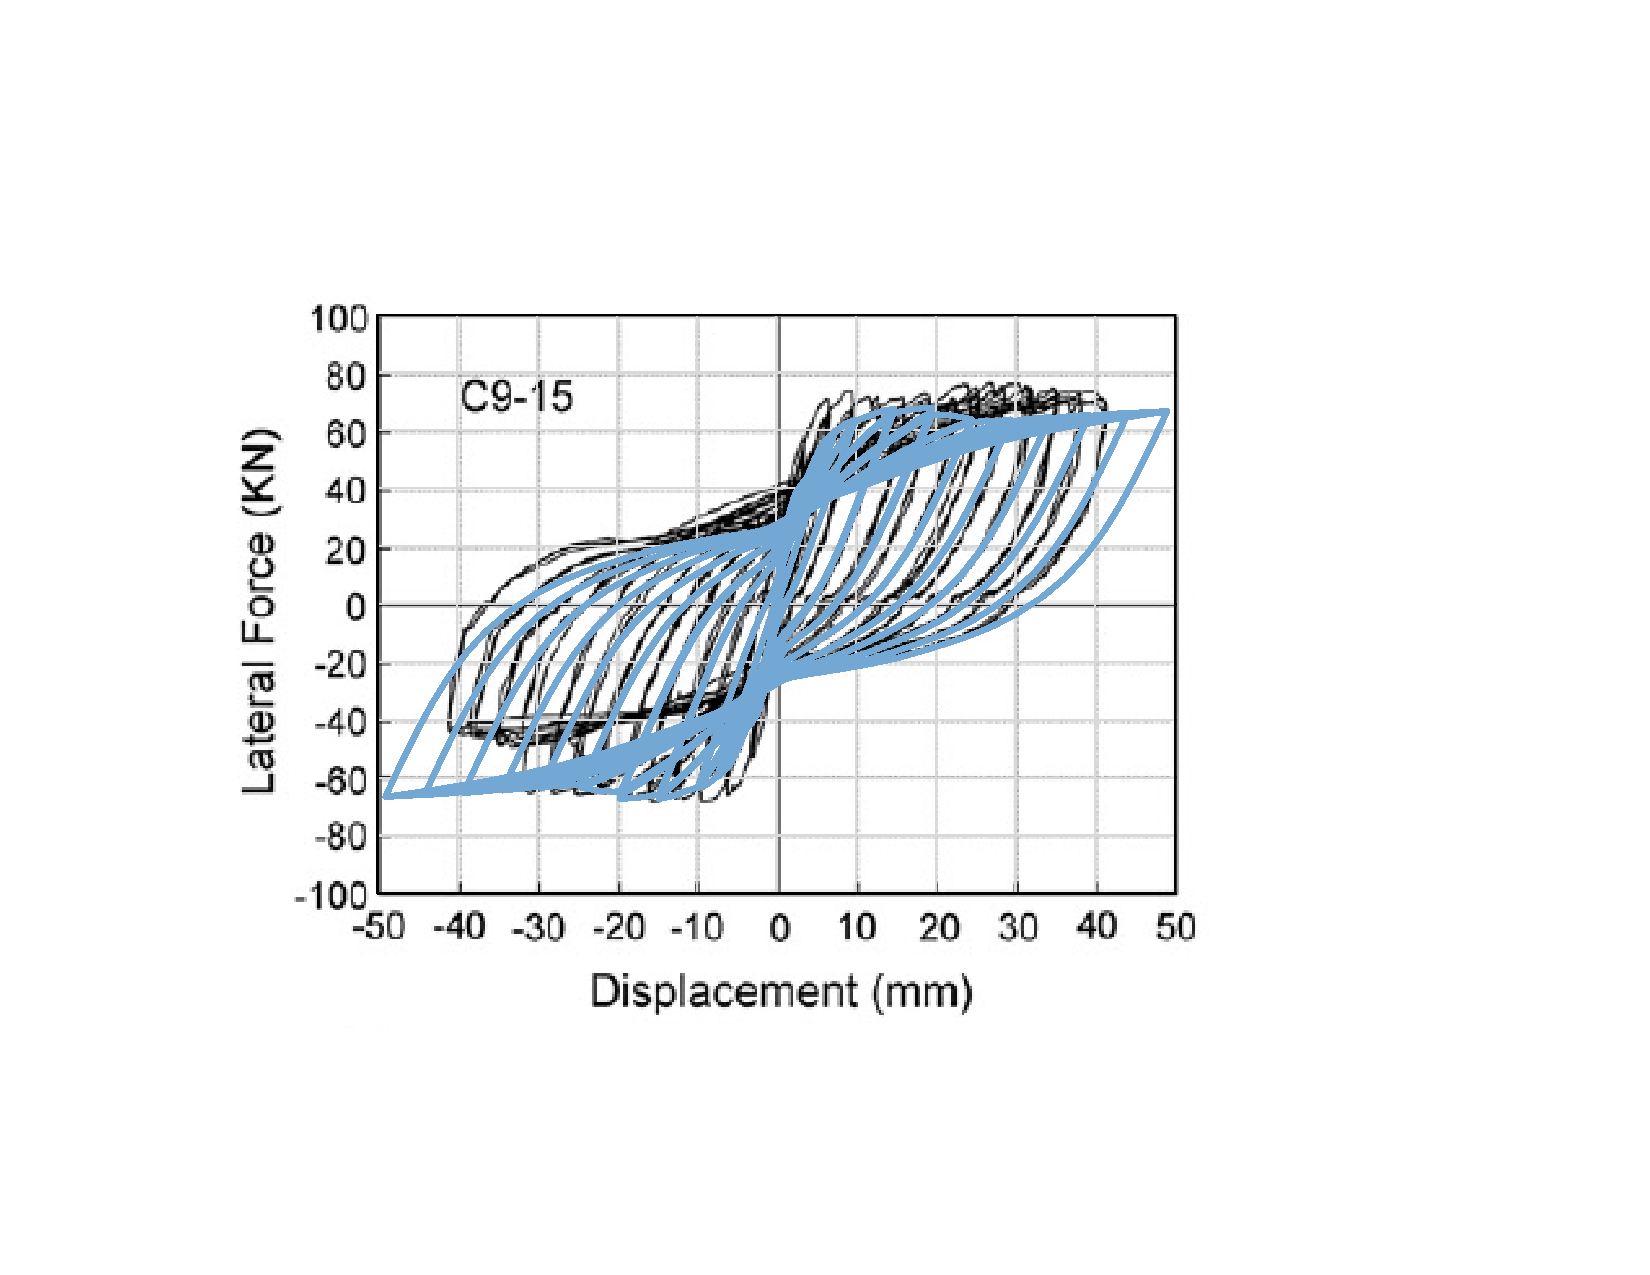
\includegraphics[width=0.60\textwidth]{Chapter-5/figs/Model_Calibration_Ma2012}
	\caption{Force-Displacement results from experimental RC column with corrosion in logitudinal bar (CL=9.5\%) \cite{Ma2012} and analytical model results (shown in lightblue)}
	\label{fig:ModelCalibration_Corrosion}
\end{figure}

Figure \ref{fig:ModelCalibration_Corrosion} shows that the results obtained from the analytical model capture the response of the structure with good accuracy. Ma et al \cite{Ma2012} did not report if bar buckling and bar fracture occurred during the test. However, the hysteresis curve shown in their study suggests that some damage limit state was reached. Therefore, \eref{eq:es_DamageControl} is used to determine the bar buckling limit state ($\varepsilon_{s,BB}=0.024$), this is then compared to the analytical model results shown \fref{fig:ModelCalibration_Corrosion_Hysteresis}. The results show a peak tension strain of $\varepsilon_{s}=0.023$, which is close to the value obtained using equation \eref{eq:es_DamageControl}. Therefore, there is a high likelihood that the bar buckling limit state was reached during this test. While these results are close, it is still not clear if \eref{eq:es_DamageControl} captures the behavior of the buckling limit state for corroded rebars. Thus, the proposed corroded BBT test will show if corrosion affects the behavior of buckled bars.

\begin{figure}[htbp]
	\centering
	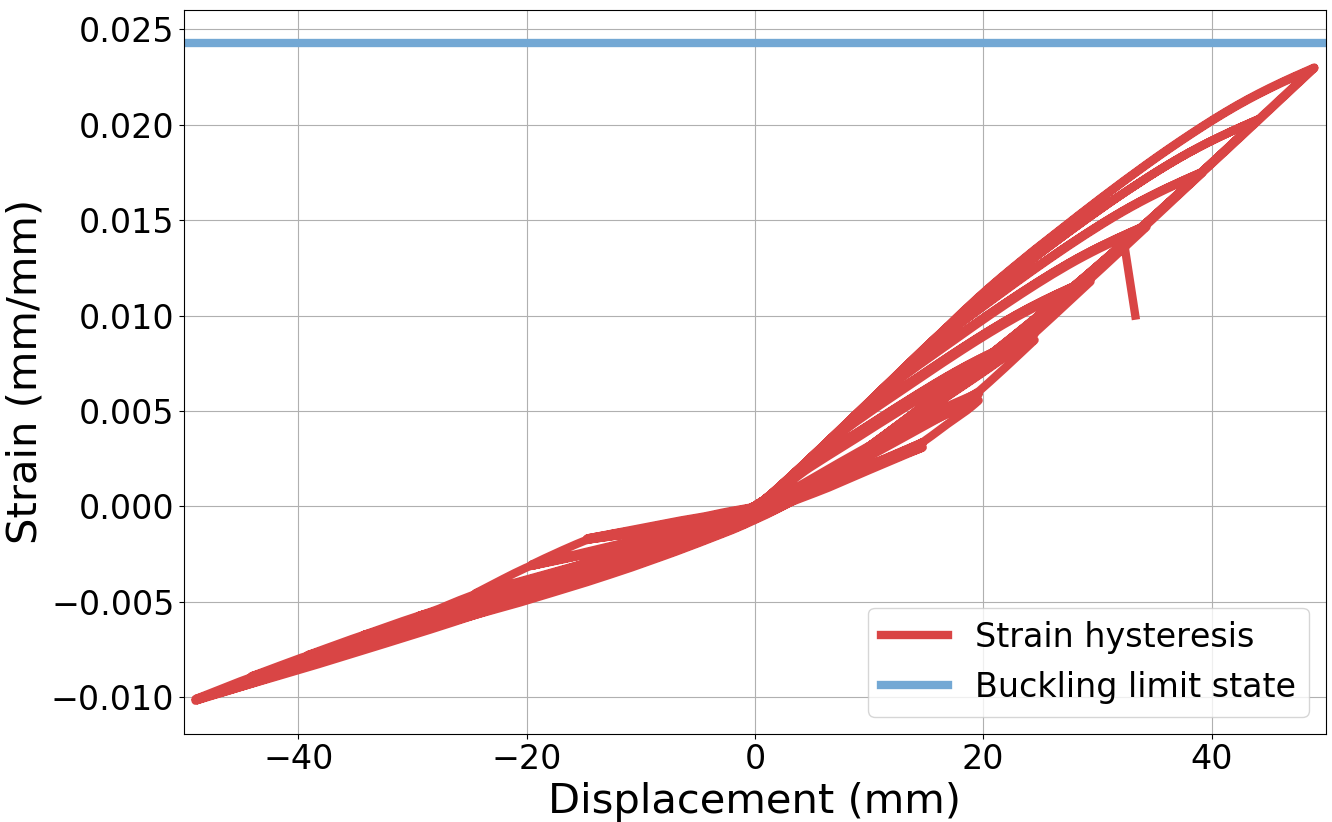
\includegraphics[width=0.6\textwidth]{Chapter-5/figs/MaEtAl_StrainHisteresis}
	\caption{Strain hysteresis from experimental RC column with corrosion in longitudinal bar (CL=9.5\%) results from analytical model}
	\label{fig:ModelCalibration_Corrosion_Hysteresis}
\end{figure}
\newpage
\section{Analytical framework}

An analytical framework is established to obtain the change in the structure performance due to aging conditions and to evaluate the effect of multiple seismic events. Therefore, a series of nonlinear time history analyses (NLTHA) will be performed. From these analyses, it is possible to determine the effects of damage in the performance of structures. The proposed analytical framework process consists of:

\begin{enumerate}
	\item Geometrical properties of the SDOF column 
	\item Properties of the material are evaluated (i.e. water to cement ratio, cover)
	\item For equal periods of time the time dependent properties are modified
	\item Nonlinear time history analyses are performed for discrete ground motions or sequence of ground motions
	\item Results are obtained and evaluated
\end{enumerate}

The analysis matrix for the corrosion aging phenomenon that will be analyzed in this study is shown in Table \ref{tab:AnalysisMatrix}. The area or extent covered in the analysis corresponds to the range of variables that are common for RC columns in bridges.

\begin{table}[htb]
	\caption{Analysis matrix}
	\label{tab:AnalysisMatrix}
	\centering
\begin{tabular}{{|l|c|c|}}
\multicolumn{3}{c}{\cellcolor[HTML]{C90000}{\color[HTML]{FFFFFF} ANALYSIS MATRIX}} \\	\hline
Description                            & Parameter        & Range                  \\	\hline
Diameter of column                     & D                & 30-90 in               \\	\hline
Column length to diameter ratio        & L/D              & 2-8                    \\	\hline
Longitudinal ratio                     & $\rho_s$         & 0.01-0.04              \\	\hline
Transverse volumetric ratio            & $\rho_v$         & 0.005-0.015            \\	\hline
Axial load ratio                       & ALR              & 0.05-0.2               \\	\hline
Water to cement ratio                  & w/c              & 0.36-0.6               \\	\hline
Cover                                  & c                & 1.5-3 in               \\	\hline
Time/condition                         & CL               & 5\%-20\%               \\	\hline
\end{tabular}
\end{table}

%This procedure has been summarized in the form of a flow chart presented in \fref{fig:NLTHA_Framework}
%
%\begin{figure}[htbp]
%	\centering
%	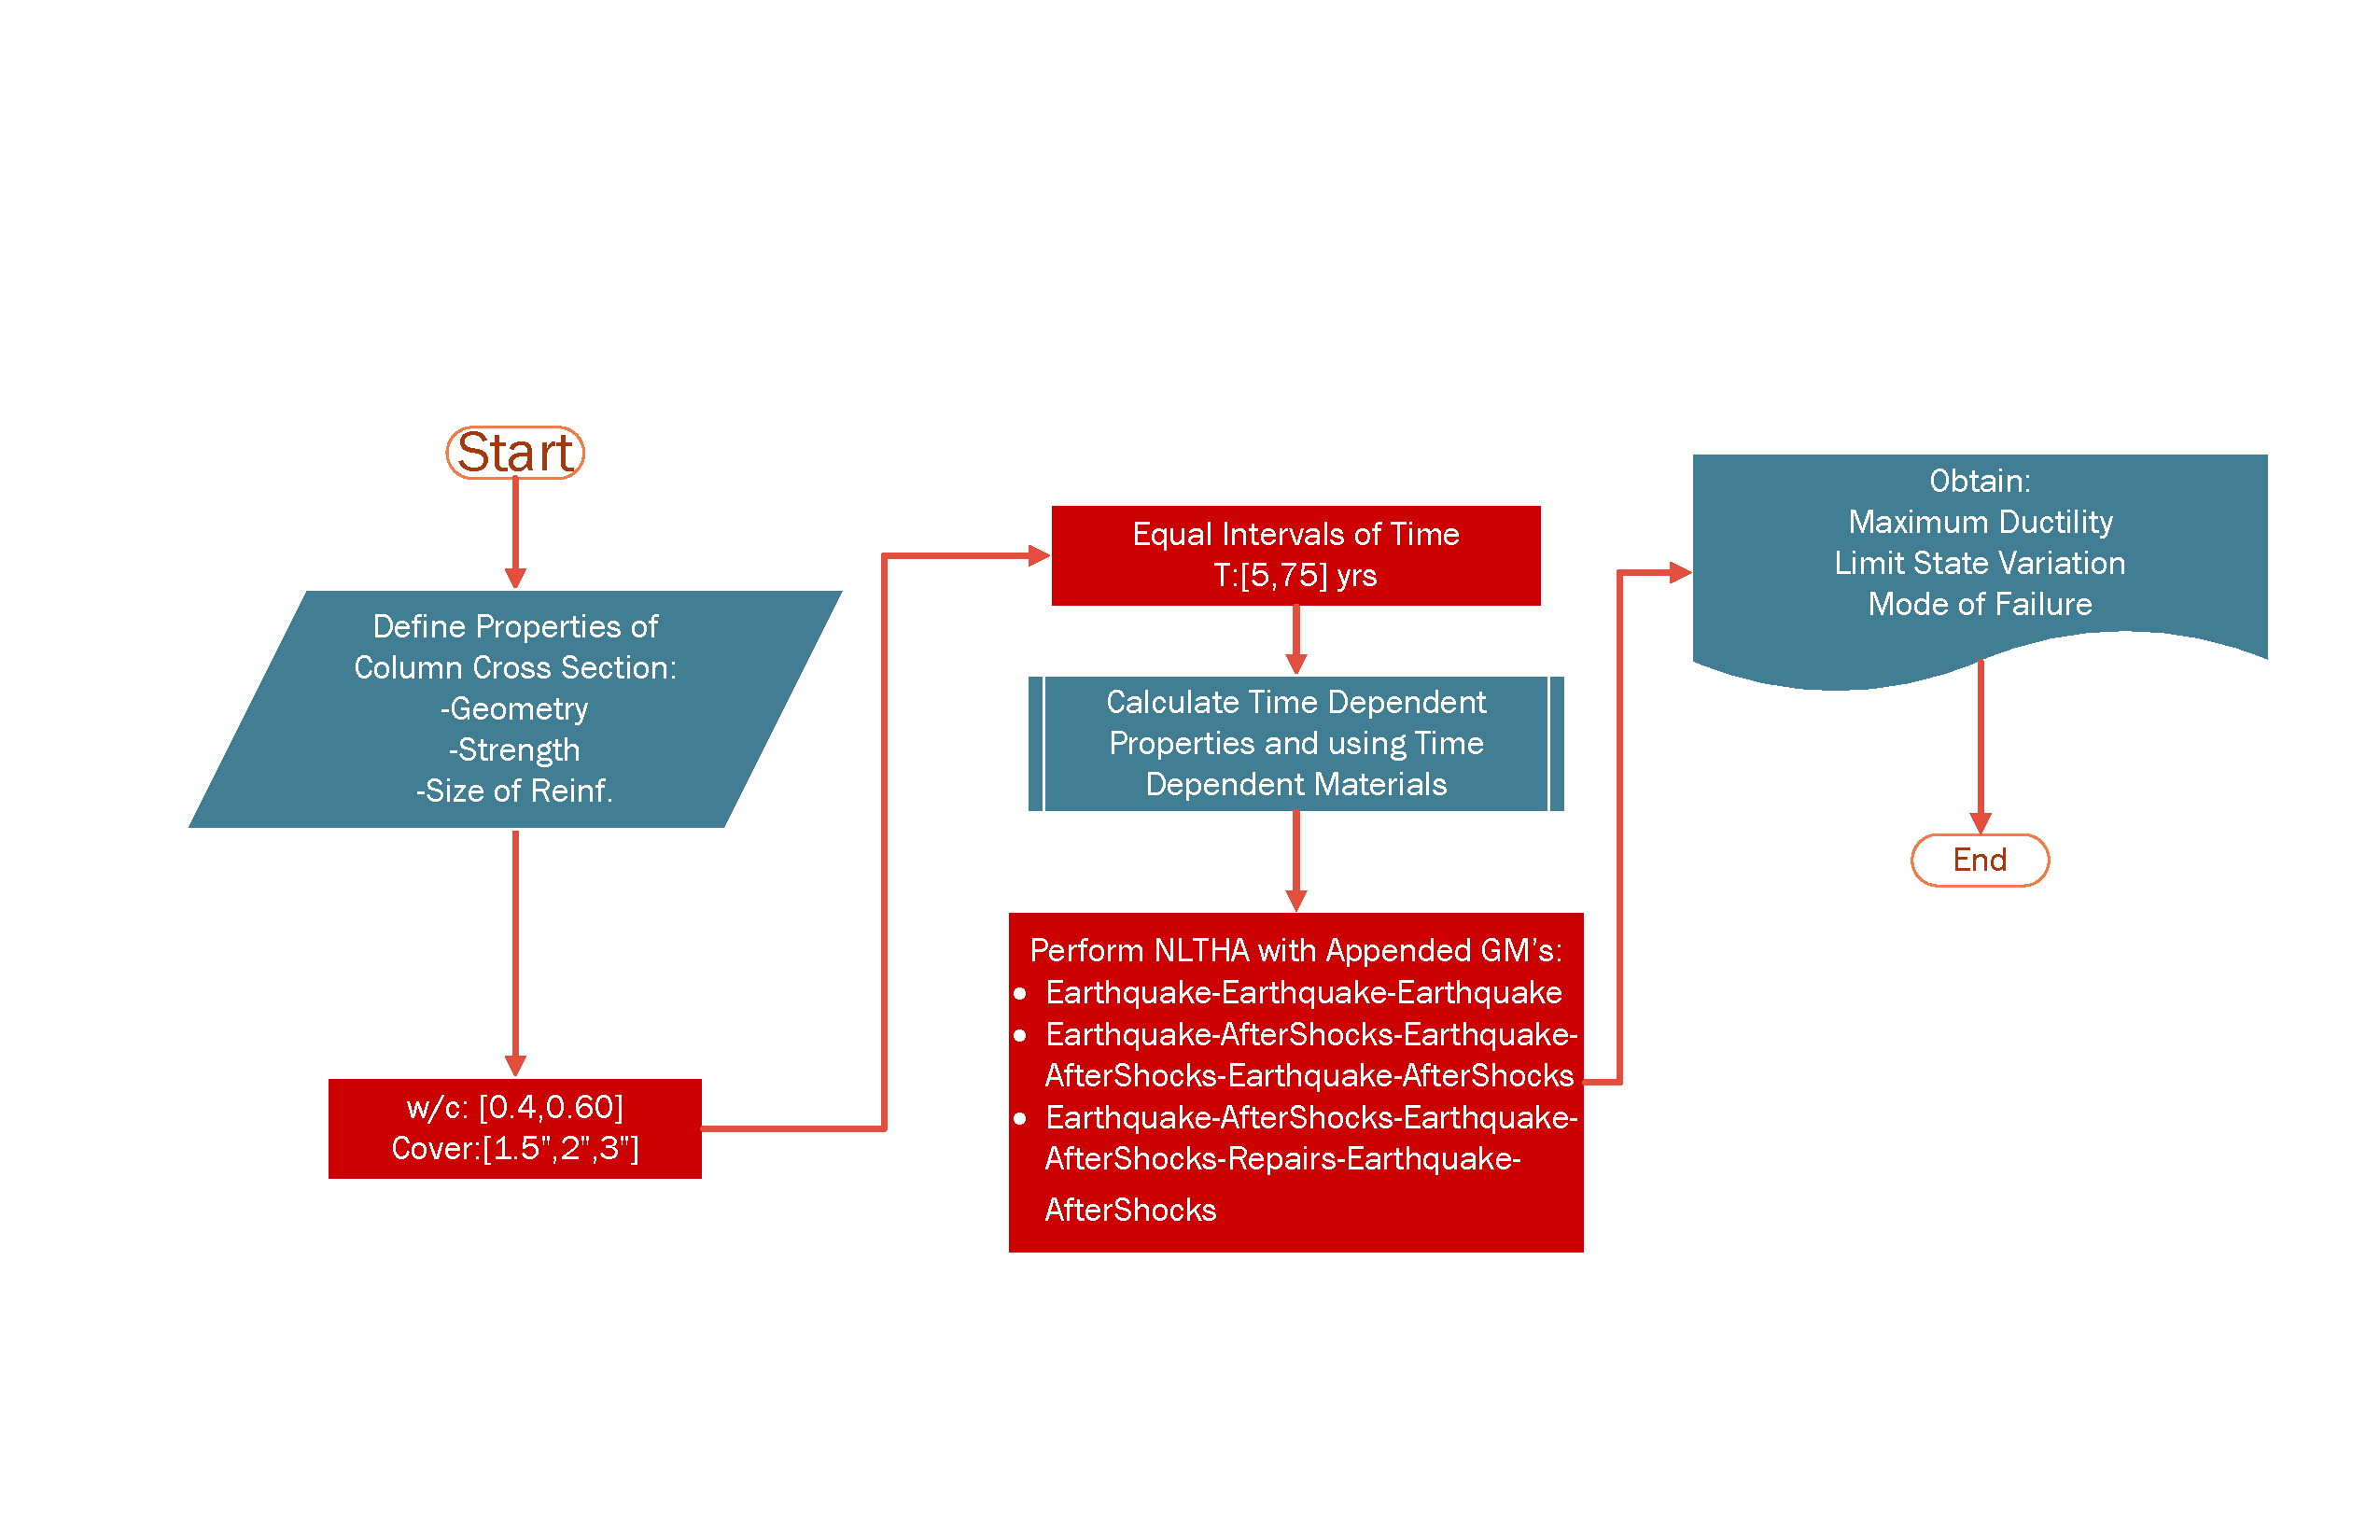
\includegraphics[width=0.9\textwidth]{Chapter-5/figs/AnalysisFramework_01}
%	\caption{Analysis Framework Flowchart}
%	\label{fig:NLTHA_Framework}
%\end{figure}
%
%\section{Earthquake selection}
%\lipsum[4]
\section{Results from NLTHA}
This section presents the results obtained from a non-linear time history analysis (NLTHA) performed using OpenSeesPy \cite{Zhu2018}. The structure was subjected to a total of 18 earthquake records. The main responses obtained from these analyses correspond to the maximum strain obtained for the different levels of corrosion. The structure was analyzed for a range of corrosion levels [1.5\%-13\%] in the longitudinal rebars.

\subsection{Effect on structure response}
Figures \ref{fig:Force-Displacement_Results} and \fref{fig:Steel_Stress_Strain_Response} are presented as an example of the results obtained using NLTHA. These results are extracted from the response of the structure to the Chi-Chi earthquake. \fref{fig:Force-Displacement_Results} shows the global system response and \fref{fig:Steel_Stress_Strain_Response} shows the stress-strain response of the extreme fiber of reinforcing steel. These results show that as corrosion increases the demands imposed on the structure increases too. Therefore, the probability of reaching a limit state increases as corrosion increases.

\begin{figure}[htbp]
	\centering
	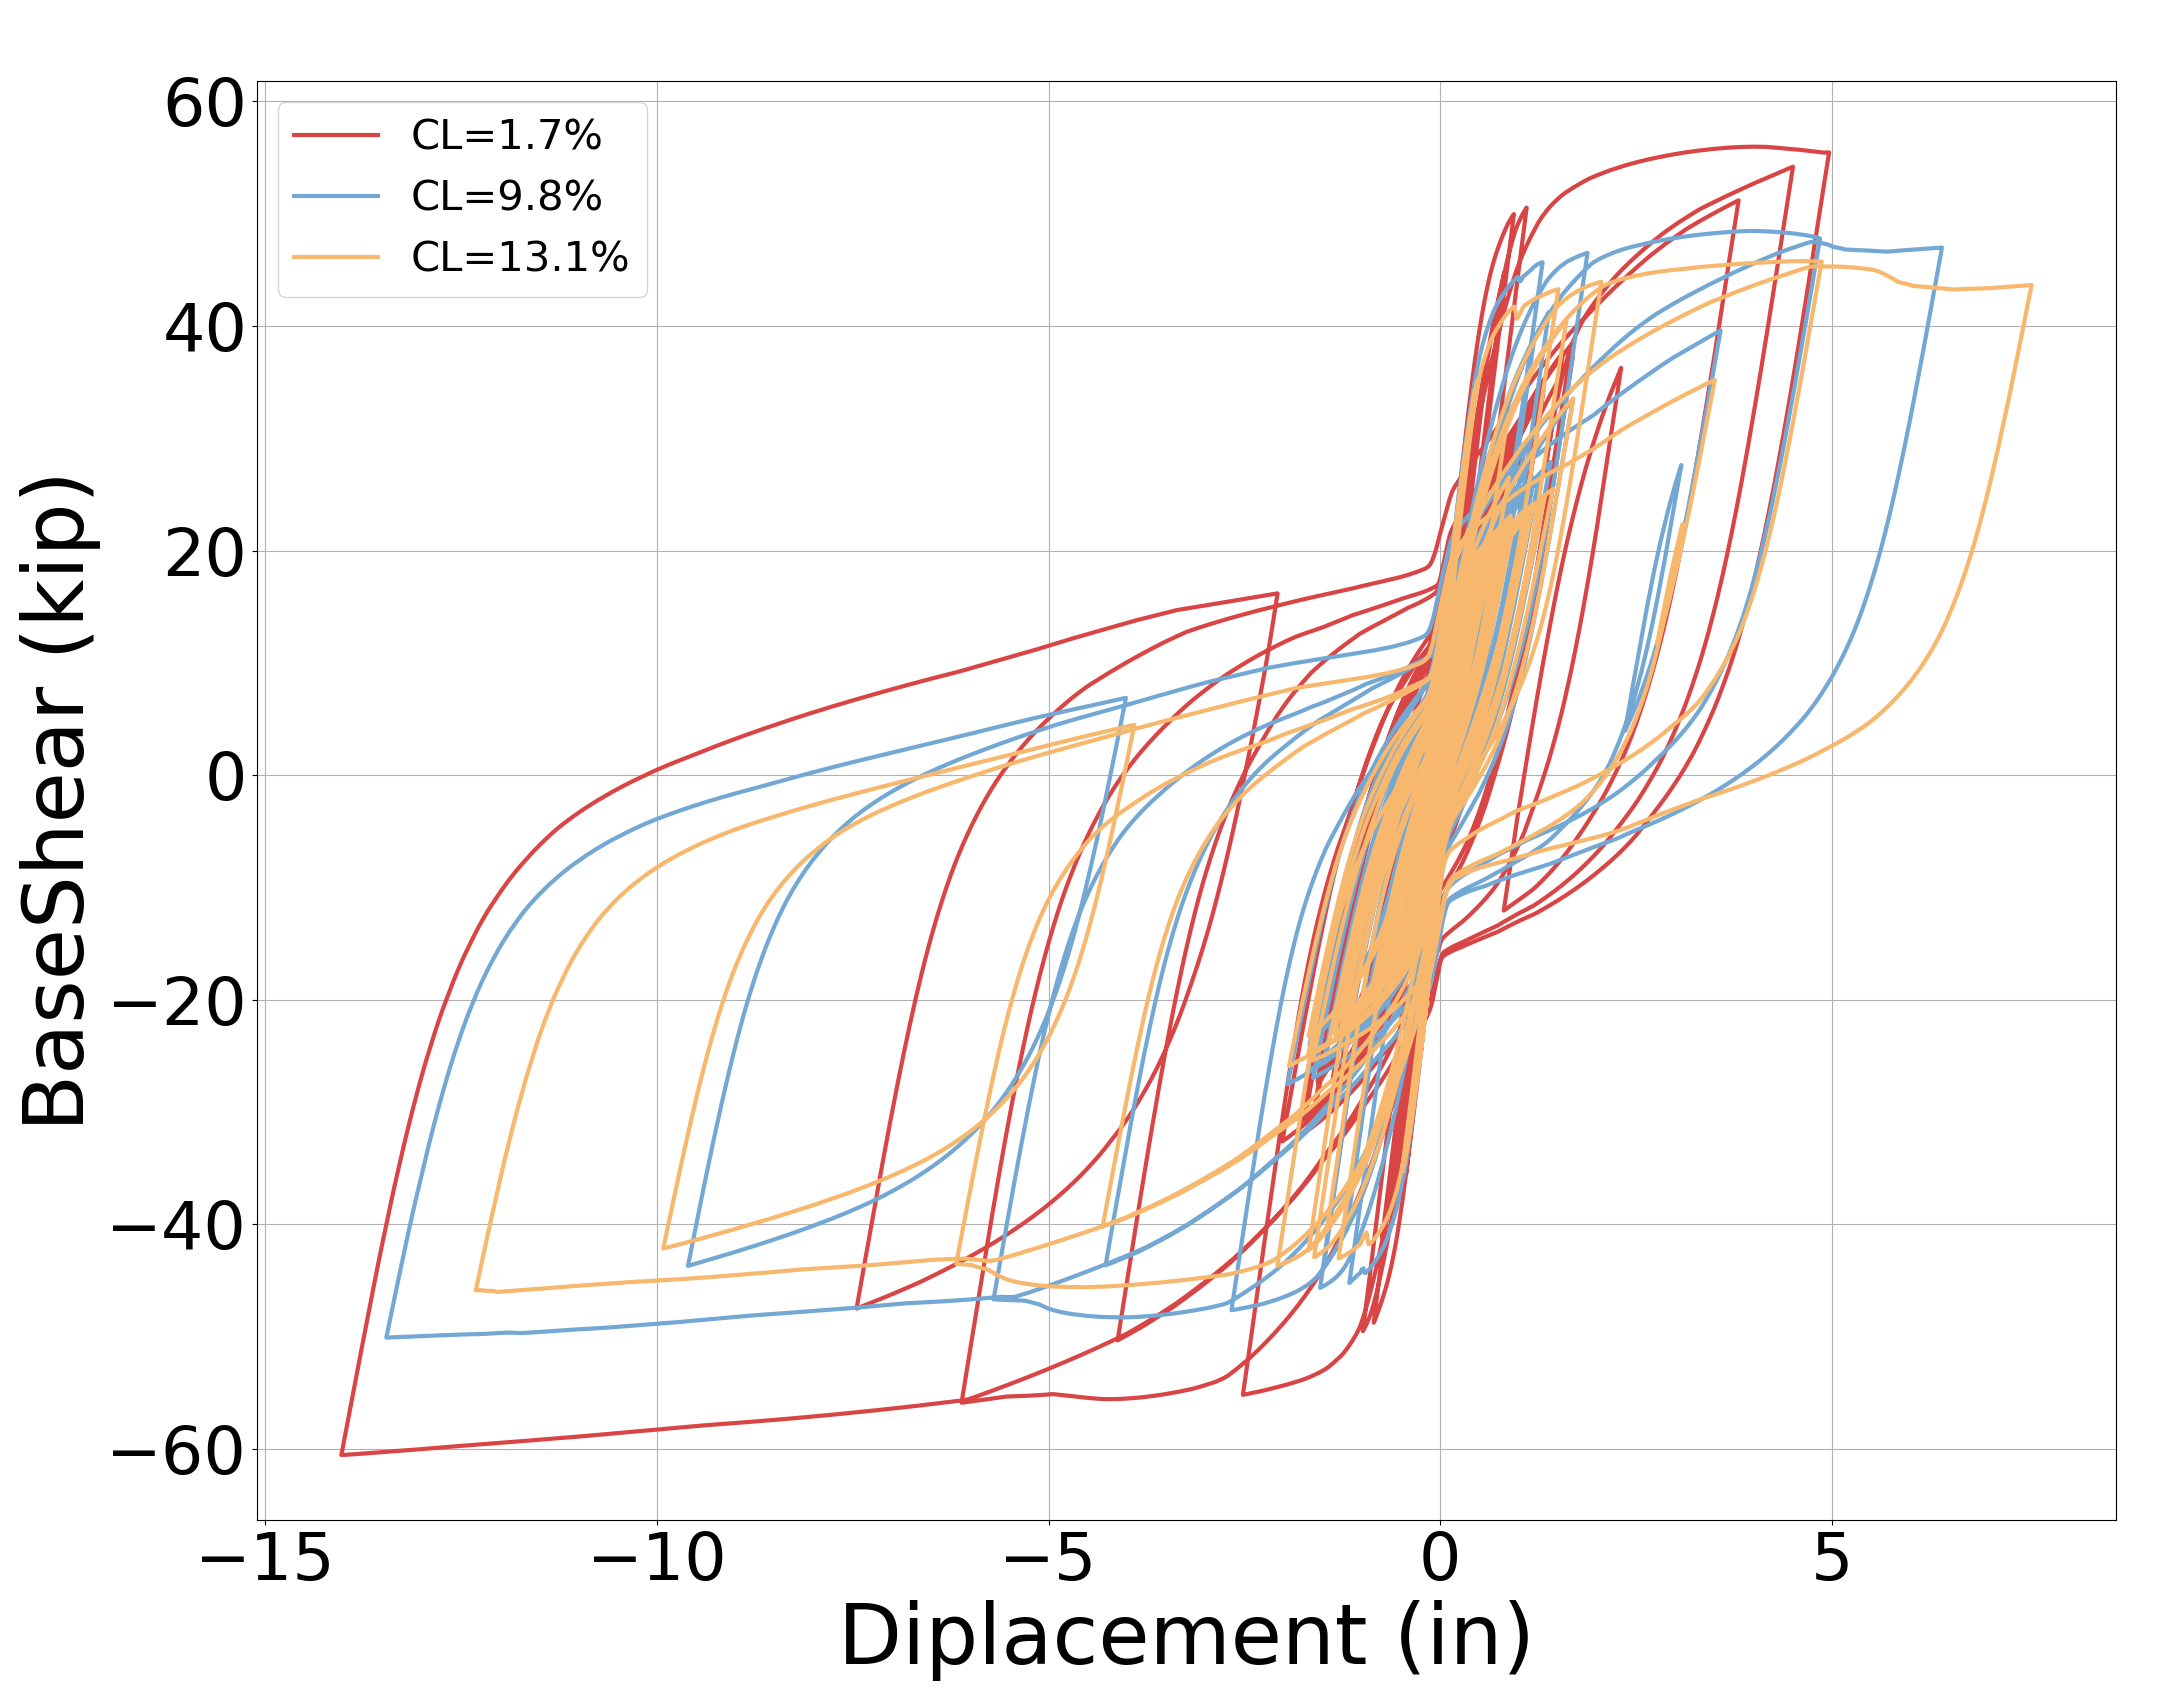
\includegraphics[width=0.65\textwidth]{Chapter-5/figs/ForceDisplacement_01}
	\caption{Force-Displacement results}
	\label{fig:Force-Displacement_Results}
\end{figure}
\begin{figure}[htbp]
	\centering
	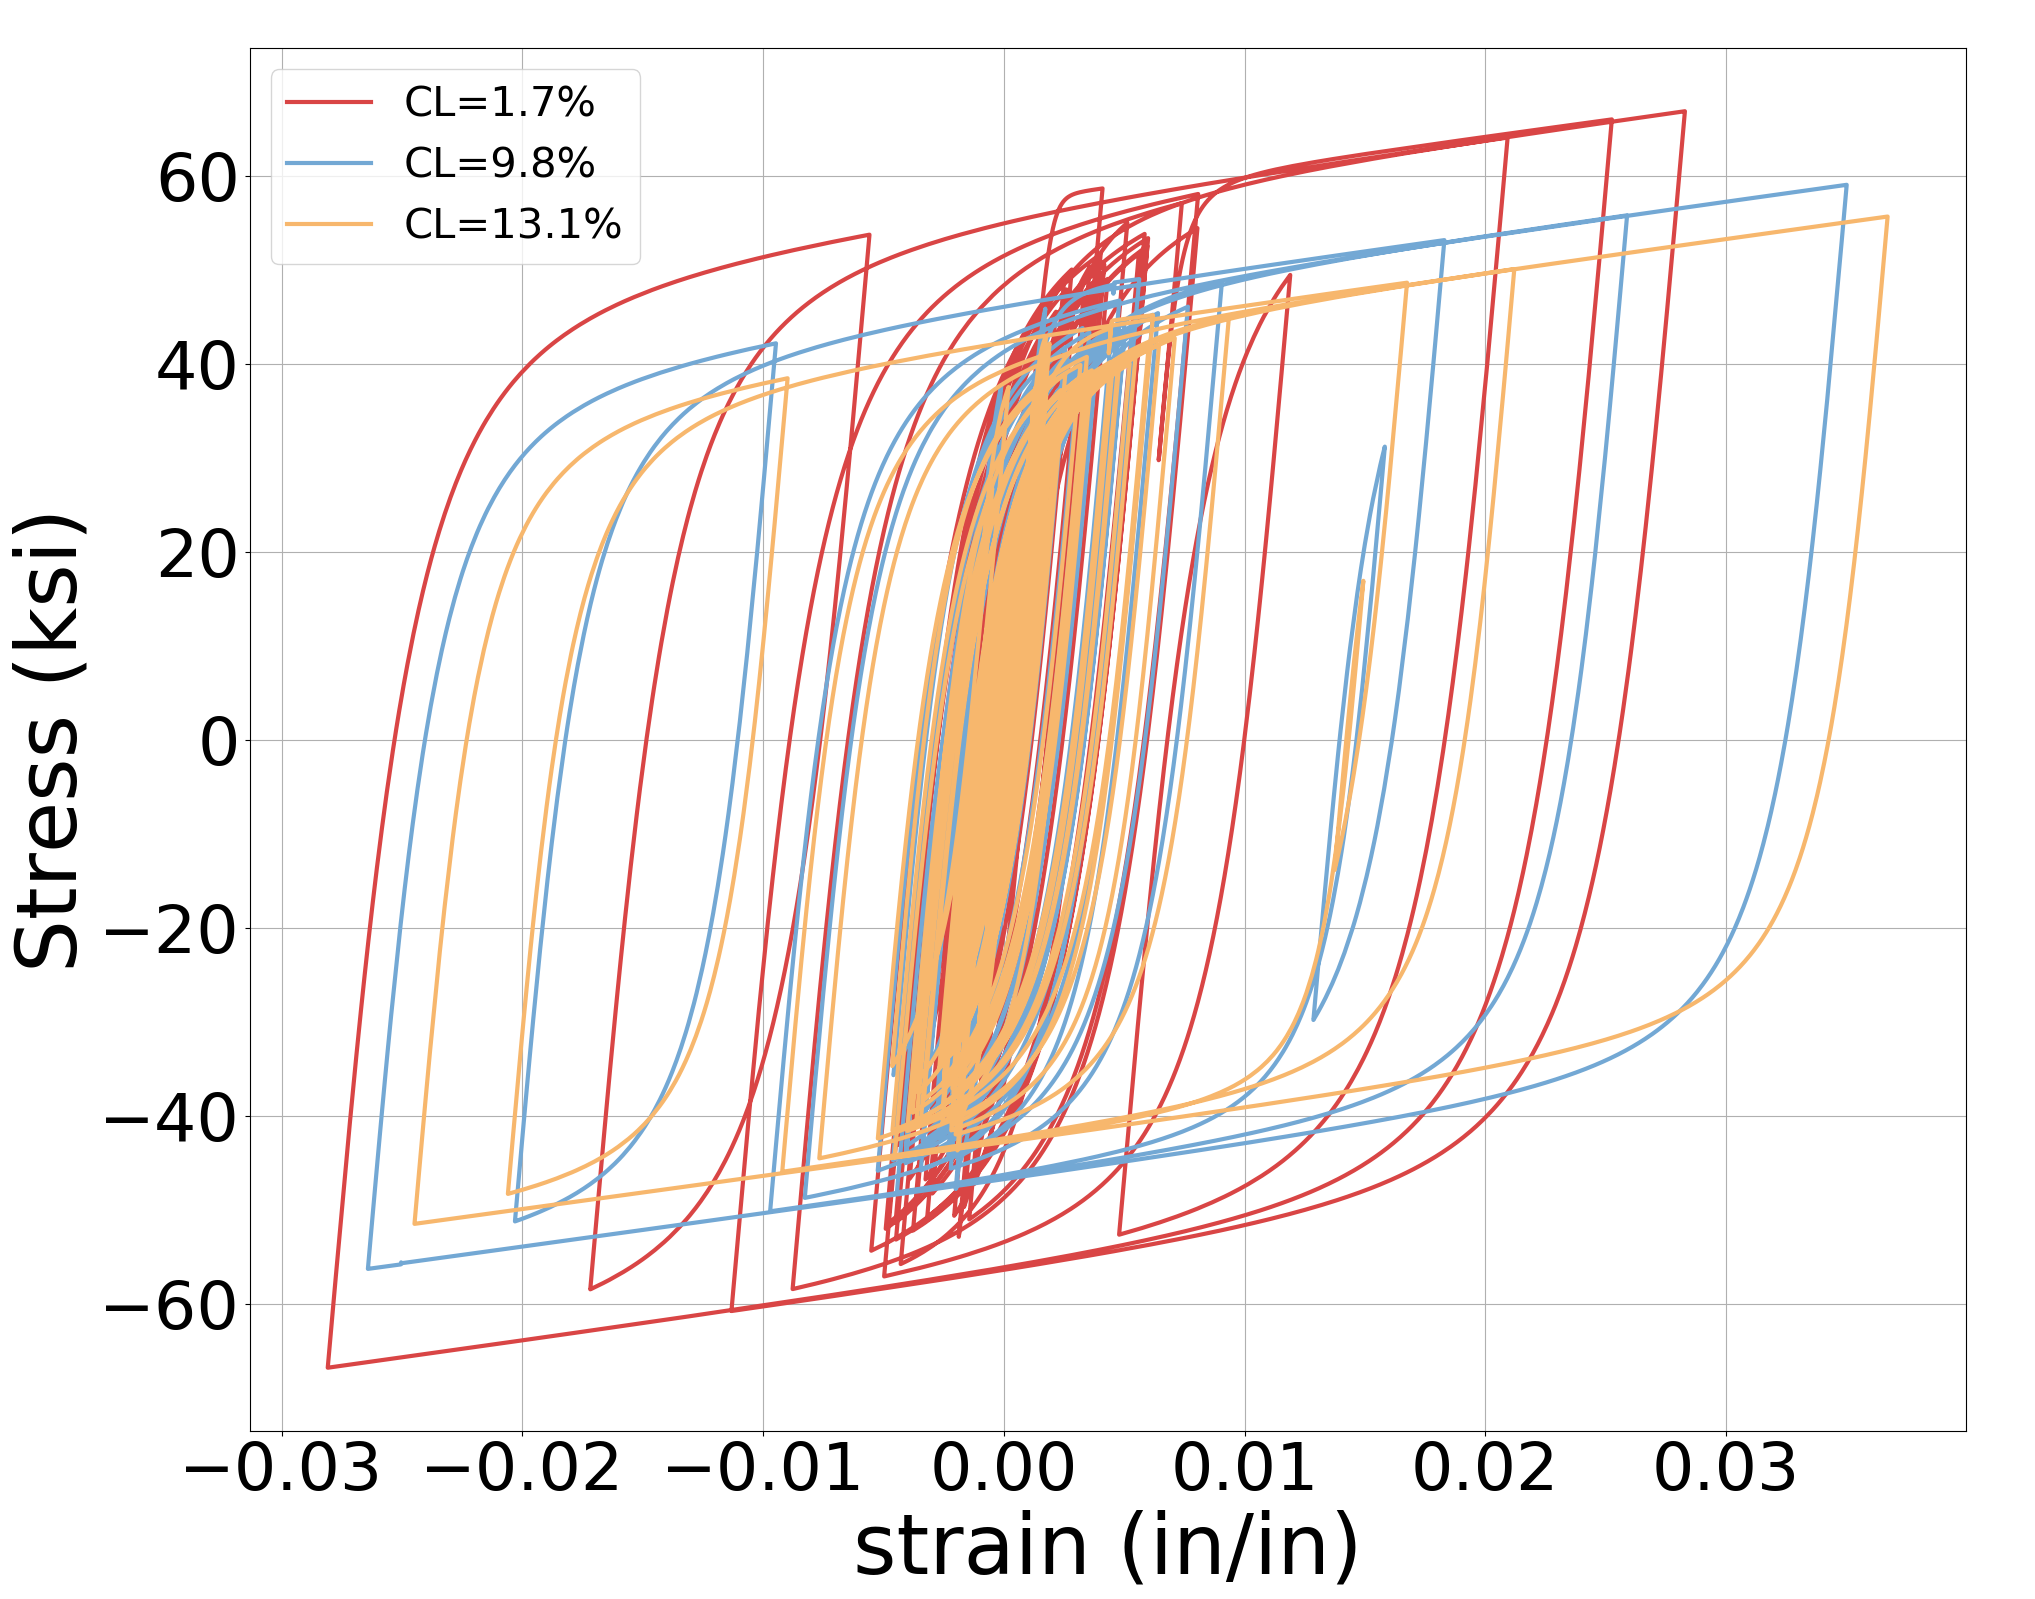
\includegraphics[width=0.65\textwidth]{Chapter-5/figs/Steel_StressStrain}
	\caption{Stress strain response for extreme rebar location}
	\label{fig:Steel_Stress_Strain_Response}
\end{figure}

\subsection{Development of cumulative distribution functions}

Once the analysis is complete the data is post-processed and expressed as a cumulative distribution function (CDF). The methodology employed corresponds to the multiple stripe analysis (MSA) recommended by Baker et al \cite{Baker2015}. While peak ground acceleration ($PGA$) has been widely used as the intensity measure to develop fragility functions\cite{Ghosh2015}\cite{Bisadi2015}\cite{Shekhar2018}. Krish \cite{Krish2018} showed in a recent study, that spectral displacement at first effective period ($IM=Sd(T_1)$) has better correlation than $PGA$. To demonstrate this, CDF curves were developed for $IM=PGA$ and $IM=Sd(T_1)$, and are shown in \fref{fig:CDF_SY_PGA} and \fref{fig:CDF_SY_SDT1} respectively. The CDFs were developed for the steel yielding limit state; however this can be the extrapolated for any limit state. \fref{fig:CDF_SY_PGA} shows the results obtained with $IM=PGA$ do not show a good correlation since as corrosion increases the probability of exceeding a limit state decreases. This is not the behavior observed in \fref{fig:Steel_Stress_Strain_Response}. Conversely, \fref{fig:CDF_SY_SDT1} shows the results with $IM=Sd(T_1)$. These results present a better correlation, since, as corrosion increases, the probability of exceeding the limit state of yielding increases. For the preliminary results shown here, the corrosion level of 13.1\% results are an exception. These results will improve as more analyses become available. 

\begin{figure}[htbp]
	\centering
	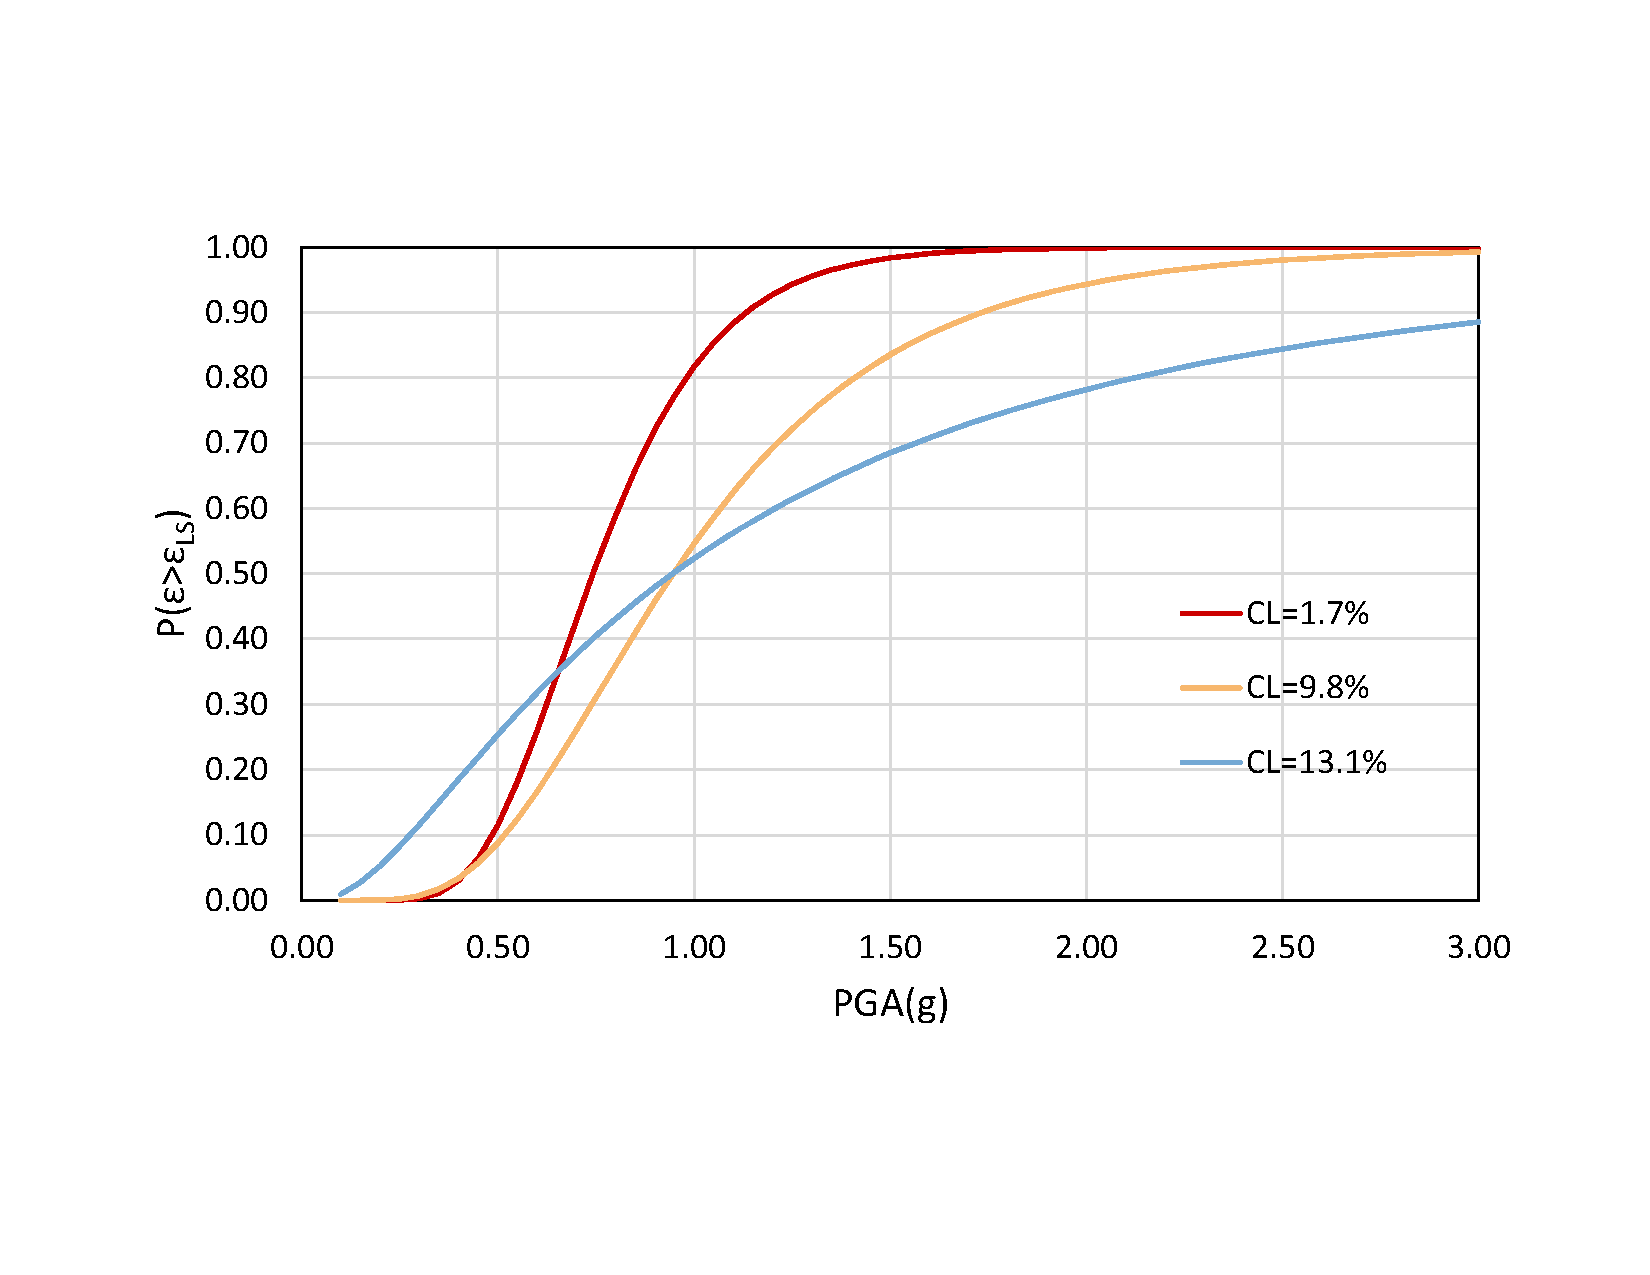
\includegraphics[width=0.8\textwidth]{Chapter-5/figs/CDF_PGA}
	\caption{CDF of steel yielding limit state using $IM=PGA$}
	\label{fig:CDF_SY_PGA}
\end{figure}
\begin{figure}[htbp]
	\centering
	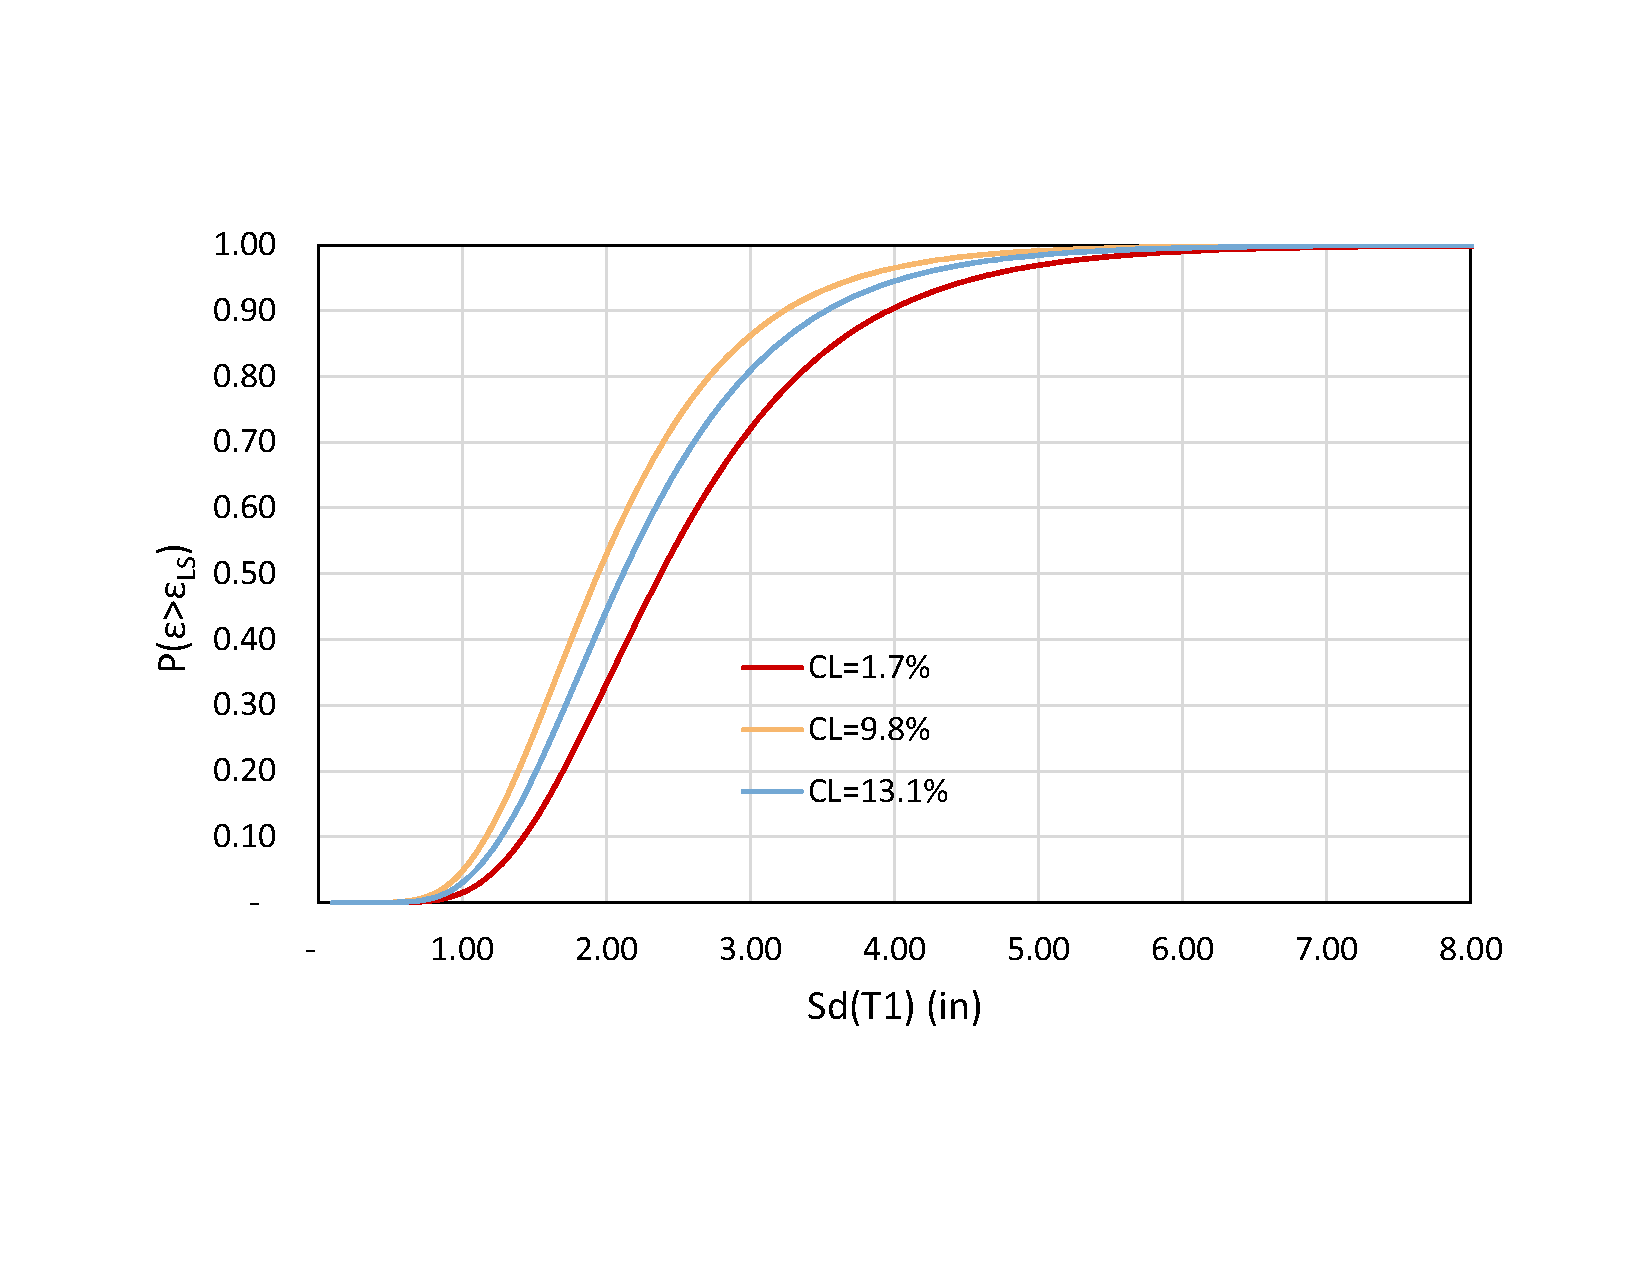
\includegraphics[width=0.8\textwidth]{Chapter-5/figs/CDF_SdT1}
	\caption{CDF of steel yielding limit state using $IM=Sd(T_1)$}
	\label{fig:CDF_SY_SDT1}
\end{figure}
\newpage
\subsection{Results discussion}
The results show that there is an increase in the demands as the corrosion in the structure increases. This is clearly shown in \fref{fig:CDF_SY_SDT1}. However, more results will help improve this correlation. In addition, the results shown in \fref{fig:CDF_SY_PGA} and \fref{fig:CDF_SY_SDT1}, demonstrate that $IM=Sd(T_1)$ is a better intensity measure than $IM=PGA$. 

Moreover, the outcomes from the experimental campaign will further improve the results obtained in the analytical work. The experimental phase will also provide an improved methodology to mimic the behavior of corroded reinforcing steel that is embedded inside the concrete, and the inclusion of additional aging conditions in the analysis will provide a realistic analysis of aging RC columns

\section{Future topics}

\begin{itemize}
	\item Strength degradation in corroded RC structures
	\item Equivalent viscous damping in corroded RC structures
	\item Selection of intensity measure (IM)
	\item Degree of damage effect on confined structures behavior
\end{itemize}